\documentclass[aspectratio=169,12pt]{beamer}
\usepackage[utf8]{inputenc}
\usepackage{amsmath, amssymb}
\usepackage{booktabs}
\usepackage{colortbl}
\usepackage{hyperref}
\usepackage{listings}
\usepackage{makecell}
\usepackage{ragged2e}
\usepackage{bytefield}
\usepackage{tikz}
\usetikzlibrary{arrows.meta, positioning, shapes.geometric, calc, tikzmark, patterns, fit, matrix, backgrounds, shapes.callouts, decorations.pathreplacing}
\usepackage{circuitikz}
\usepackage{verbatim}  % For comment environment
\usetheme{Madrid}

% Pseudocode listing style
\lstdefinestyle{pseudocode}{
    basicstyle=\ttfamily\small,
    keywordstyle=\bfseries\color{blue!70!black},
    commentstyle=\color{green!50!black},
    stringstyle=\color{red!70!black},
    showstringspaces=false,
    numbers=none,
    frame=single,
    backgroundcolor=\color{gray!10},
    breaklines=true,
    morekeywords={if, else, return, while, for, def, and, or, not},
    morecomment=[l]{//},
}

% Define colors for registers
\definecolor{r1color}{RGB}{255,0,0}
\definecolor{r2color}{RGB}{0,128,0}
\definecolor{r3color}{RGB}{255,165,0}
\definecolor{r4color}{RGB}{128,0,128}
\definecolor{r5color}{RGB}{0,0,255}
\definecolor{r6color}{RGB}{255,165,0}
\definecolor{r7color}{RGB}{0,0,0}
\definecolor{r8color}{RGB}{0,128,0}

% Define hyphenation command
\newcommand{\hyp}{\-}

% Address breakdown command from recitation
\newcommand{\addressbreakdown}[3]{%
    \begin{tikzpicture}[
        section/.style={draw, very thick, minimum height=0.6cm},
        bitnumber/.style={font=\tiny},
        sectionlabel/.style={font=\scriptsize},
        baseline=(current bounding box.center)
    ]
    % Calculate total bits and positions
    \pgfmathtruncatemacro{\totalbits}{#1 + #2 + #3}
    \pgfmathtruncatemacro{\tagstart}{\totalbits - 1}
    \pgfmathtruncatemacro{\tagend}{\totalbits - #1}
    \pgfmathtruncatemacro{\setstart}{\tagend - 1}
    \pgfmathtruncatemacro{\setend}{\tagend - #2}
    \pgfmathtruncatemacro{\offsetstart}{\setend - 1}
    \pgfmathtruncatemacro{\offsetend}{0}
    
    % Scale factor for width (adjust this to change overall size)
    \pgfmathsetmacro{\bitwidth}{0.17}
    
    % Starting position
    \pgfmathsetmacro{\xpos}{0}
    
    % Draw tag block
    \ifnum#1>0
        \pgfmathsetmacro{\tagwidth}{#1 * \bitwidth}
        \node[section, fill=blue!40, minimum width=\tagwidth cm] (tag) at (\xpos + \tagwidth/2, 0) {};
        \node[sectionlabel] at (tag.center) {tag};
        
        % Add bit numbers below
        \node[bitnumber] at ($(tag.south west) + (0mm,-1mm)$) {\tagstart};
        \node[bitnumber] at ($(tag.south east) + (-1mm,-1mm)$) {\tagend};
        
        \pgfmathsetmacro{\xpos}{\xpos + \tagwidth}
    \fi
    
    % Draw set block
    \ifnum#2>0
        \pgfmathsetmacro{\setwidth}{#2 * \bitwidth}
        \node[section, fill=green!40, minimum width=\setwidth cm] (set) at (\xpos + \setwidth/2, 0) {};
        % if num is smaller than 2 rotate label
        \ifnum#2<3
            \node[sectionlabel, rotate=90] at (set.center) {set};
        \else
            \node[sectionlabel] at (set.center) {set};
        \fi
        % Add bit numbers below
        \node[bitnumber] at ($(set.south west) + (1mm,-1mm)$) {\setstart};
        \node[bitnumber] at ($(set.south east) + (-1mm,-1mm)$) {\setend};
        
        \pgfmathsetmacro{\xpos}{\xpos + \setwidth}
    \fi
    
    % Draw offset block
    \ifnum#3>0
        \pgfmathsetmacro{\offsetwidth}{#3 * \bitwidth}
        \node[section, fill=yellow!40, minimum width=\offsetwidth cm] (offset) at (\xpos + \offsetwidth/2, 0) {};
        \ifnum#3<3
            \node[sectionlabel, rotate=90, font=\tiny] at (offset.center) {offset};
        \else
            \node[sectionlabel] at (offset.center) {offset};
        \fi
        
        % Add bit numbers below
        \node[bitnumber] at ($(offset.south west) + (1mm,-1mm)$) {\offsetstart};
        \node[bitnumber] at ($(offset.south east) + (0mm,-1mm)$) {\offsetend};
    \fi
    \end{tikzpicture}
}

% Proportional widths for the table-only version
\newlength\TotalW
\setlength\TotalW{\textwidth}
\newlength\Wone    \setlength\Wone   {0.015625\TotalW} % 1/64
\newlength\Weleven \setlength\Weleven{0.171875\TotalW} % 11/64
\newlength\Wforty  \setlength\Wforty {0.625000\TotalW} % 40/64
\newlength\Wtwelve \setlength\Wtwelve{0.187500\TotalW} % 12/64
\newcolumntype{L}[1]{>{\RaggedRight\arraybackslash}p{#1}}
\newcolumntype{C}[1]{>{\Centering\arraybackslash}p{#1}}
\renewcommand{\arraystretch}{1.2}

\title{Virtual Memory}
\author{Computer Architecture 2360267}
\date{2025, Lecture \#9}
\begin{document}

\frame{\titlepage}

% Table of Contents
\begin{frame}{Outline}
\tableofcontents
\end{frame}

\section{Introduction to Virtual Memory}

\begin{frame}{Virtual Memory}
\begin{itemize}
\item \textbf{Provide isolation:} each process sees its own memory space
    \begin{itemize}
    \item Many processes can run on a single machine
    \item Prevents a process from accessing the memory of other processes
    \end{itemize}
\item \textbf{Provides the illusion of a large memory for each process}
    \begin{itemize}
    \item Different machines have different amount of physical memory
    \item Allows programs to run regardless of actual physical memory size
    \item Sum of memory spaces of all process may be larger than physical memory
    \end{itemize}
\item \textbf{Provides illusion of contiguous memory}
    \begin{itemize}
    \item The amount of memory consumed by each process is dynamic
    \item Allows adding memory and keep it contiguous
    \end{itemize}
\end{itemize}
\end{frame}

\begin{frame}{Virtual Address Spaces}
\begin{center}
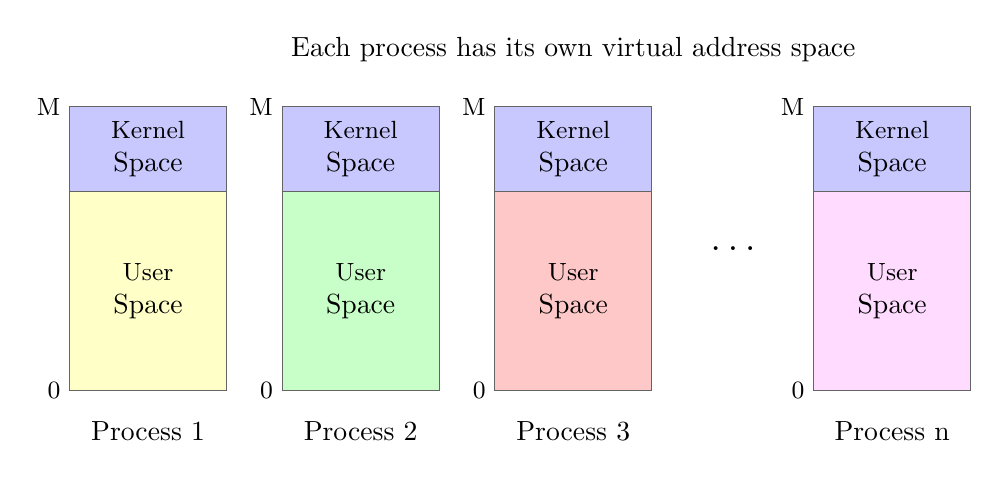
\begin{tikzpicture}[scale=0.9]
    % Define colors
    \definecolor{kernelcolor}{RGB}{200,200,255}
    \definecolor{usercolor1}{RGB}{255,255,200}
    \definecolor{usercolor2}{RGB}{200,255,200}
    \definecolor{usercolor3}{RGB}{255,200,200}
    \definecolor{usercolor4}{RGB}{255,220,255}
    \definecolor{bordercolor}{RGB}{100,100,100}
    
    % Define dimensions
    \def\procwidth{2.2}
    \def\procheight{4}
    \def\kernelheight{1.2}
    \def\spacing{0.8}
    \pgfmathsetmacro{\kernelcenter}{\procheight-\kernelheight/2}
    \pgfmathsetmacro{\usercenter}{(\procheight-\kernelheight)/2}
    
    % Draw processes using foreach loop
    \foreach \i in {0, 1, 2} {
        \begin{scope}[shift={({\i*(\procwidth+\spacing)},0)}]
            \draw[thick, bordercolor] (0,0) rectangle (\procwidth,\procheight);
            
            % Kernel space (top)
            \fill[kernelcolor] (0,\procheight-\kernelheight) rectangle (\procwidth,\procheight);
            \draw[thick, bordercolor] (0,\procheight-\kernelheight) -- (\procwidth,\procheight-\kernelheight);
            
            % User space (bottom) - different color for each process
            \pgfmathtruncatemacro{\colornum}{\i+1}
            \fill[usercolor\colornum] (0,0) rectangle (\procwidth,\procheight-\kernelheight);
            
            % Labels with two lines
            \node[align=center] at (\procwidth/2, \kernelcenter) {\small Kernel\\Space};
            \node[align=center] at (\procwidth/2, \usercenter) {\small User\\Space};
            
            % Address labels
            \node[left] at (0, \procheight) {\small M};
            \node[left] at (0, 0) {\small 0};
            
            % Process label
            \pgfmathtruncatemacro{\procnum}{\i+1}
            \node[below] at (\procwidth/2, -0.3) {Process \procnum};
        \end{scope}
    }
    
    % Dots indicating more processes
    \node at ({{3*(\procwidth+\spacing) + \spacing/2}}, \procheight/2) {\Large \ldots};
    
    % Process n
    \begin{scope}[shift={({3.5*(\procwidth+\spacing)},0)}]
        \draw[thick, bordercolor] (0,0) rectangle (\procwidth,\procheight);
        
        % Kernel space (top)
        \fill[kernelcolor] (0,\procheight-\kernelheight) rectangle (\procwidth,\procheight);
        \draw[thick, bordercolor] (0,\procheight-\kernelheight) -- (\procwidth,\procheight-\kernelheight);
        
        % User space (bottom) - use color 4 for process n
        \fill[usercolor4] (0,0) rectangle (\procwidth,\procheight-\kernelheight);
        
        % Labels with two lines
        \node[align=center] at (\procwidth/2, \kernelcenter) {\small Kernel\\Space};
        \node[align=center] at (\procwidth/2, \usercenter) {\small User\\Space};
        
        % Address labels
        \node[left] at (0, \procheight) {\small M};
        \node[left] at (0, 0) {\small 0};
        
        % Process label
        \node[below] at (\procwidth/2, -0.3) {Process n};
    \end{scope}
    
    % Title/description
    \node[above, font=\normalsize] at ({2.5*\procwidth + 2*\spacing}, \procheight + 0.5) {Each process has its own virtual address space};
    
\end{tikzpicture}
\end{center}
\end{frame}

\begin{frame}{Virtual Memory: Basic Idea}
\begin{itemize}
\item \textbf{Basic terminology}
    \begin{itemize}
    \item Virtual Address Space (per process): address space used by the process
    \item Physical Address: actual physical memory address space
    \end{itemize}
\item \textbf{Divide each space (virtual and physical) into fixed size blocks}
    \begin{itemize}
    \item Pages in Virtual space, Frames in Physical space
    \item Page size = Frame size = some power of 2
    \end{itemize}
\item \textbf{Virtual pages are mapped either to}
    \begin{itemize}
    \item A physical frame in memory
    \item Or a sector in the disk
    \end{itemize}
\item \textbf{All addresses in programs use Virtual Memory Address Space}
    \begin{itemize}
    \item Hardware translates virtual to physical addresses on-the-fly
    \item Uses a Page Table for the translation
    \end{itemize}
\end{itemize}
\end{frame}

\section{Page Tables and Address Translation}

\begin{frame}{Page Tables}
\begin{columns}[T]
\column{0.28\textwidth}
\small
\begin{itemize}
\item OS manages a page table per process
\item Maps virtual pages to physical pages or disk
\item Only OS writes to page tables
\item Page tables reside in DRAM
\end{itemize}

\column{0.72\textwidth}
\centering
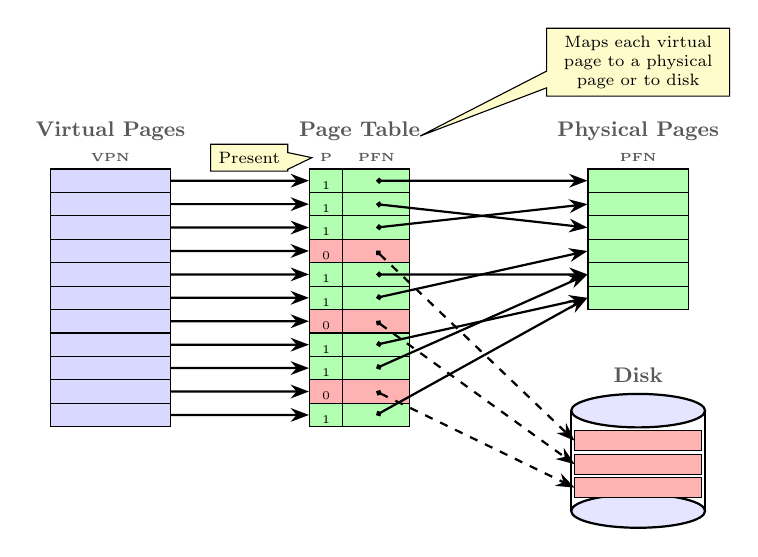
\begin{tikzpicture}[scale=0.85, every node/.style={scale=0.85},
    % Base style for all table cells
    cell/.style={draw, minimum height=0.35cm, inner sep=0pt, font=\tiny, text depth=0pt, text height=0.25cm, anchor=center},
    % Virtual pages
    vpage/.style={cell, fill=blue!15, minimum width=1.8cm},
    % Page table - present bit column
    ptgreen/.style={cell, fill=green!30, minimum width=0.5cm},
    ptred/.style={cell, fill=red!30, minimum width=0.5cm},
    % Page table - PFN column
    ptdatagreen/.style={cell, fill=green!30, minimum width=1cm},
    ptdatared/.style={cell, fill=red!30, minimum width=1cm},
    % Physical pages
    ppage/.style={cell, fill=green!30, minimum width=1.5cm},
    % Labels
    mytitle/.style={font=\small\bfseries, text=gray!70!black},
    colheader/.style={font=\tiny\bfseries, text=gray!70!black, minimum height=0.3cm},
    arrow/.style={-Stealth, thick},
    dotarrow/.style={{Circle[length=2pt]}-Stealth, thick}
]

% Virtual Pages
\matrix[matrix of nodes, row sep=-\pgflinewidth, ampersand replacement=\&,
    label={[mytitle, label distance=-2mm]above:Virtual Pages}] (vp) {
    |[colheader]| VPN \\
    |[vpage]| \phantom{x} \\
    |[vpage]| \phantom{x} \\
    |[vpage]| \phantom{x} \\
    |[vpage]| \phantom{x} \\
    |[vpage]| \phantom{x} \\
    |[vpage]| \phantom{x} \\
    |[vpage]| \phantom{x} \\
    |[vpage]| \phantom{x} \\
    |[vpage]| \phantom{x} \\
    |[vpage]| \phantom{x} \\
    |[vpage]| \phantom{x} \\
};

% Page Table - positioned relative to vp
\matrix[matrix of nodes, row sep=-\pgflinewidth, column sep=-\pgflinewidth, ampersand replacement=\&,
    right=1.5cm of vp, anchor=north west,
    label={[mytitle, label distance=-2mm]above:Page Table}] (pt) at (vp.north east) {
    |[colheader]| P \& |[colheader]| PFN \\
    |[ptgreen]| 1 \& |[ptdatagreen]| \\
    |[ptgreen]| 1 \& |[ptdatagreen]| \\
    |[ptgreen]| 1 \& |[ptdatagreen]| \\
    |[ptred]| 0 \& |[ptdatared]| \\
    |[ptgreen]| 1 \& |[ptdatagreen]| \\
    |[ptgreen]| 1 \& |[ptdatagreen]| \\
    |[ptred]| 0 \& |[ptdatared]| \\
    |[ptgreen]| 1 \& |[ptdatagreen]| \\
    |[ptgreen]| 1 \& |[ptdatagreen]| \\
    |[ptred]| 0 \& |[ptdatared]| \\
    |[ptgreen]| 1 \& |[ptdatagreen]| \\
};

% Physical Pages - positioned relative to pt
\matrix[matrix of nodes, row sep=-\pgflinewidth, ampersand replacement=\&,
    right=2cm of pt, anchor=north west,
    label={[mytitle, label distance=-2mm]above:Physical Pages}] (pp) at (pt.north east) {
    |[colheader]| PFN \\
    |[ppage]| \phantom{x} \\
    |[ppage]| \phantom{x} \\
    |[ppage]| \phantom{x} \\
    |[ppage]| \phantom{x} \\
    |[ppage]| \phantom{x} \\
    |[ppage]| \phantom{x} \\
};

% Page Table callout description - above Physical Pages
\node[rectangle callout, draw, fill=yellow!20, callout absolute pointer={(pt.north east)},
    font=\scriptsize, text width=2.5cm, align=center, above=0.5cm of pp.north] (ptdesc)
    {Maps each virtual page to a physical page or to disk};

% Present bit callout
\node[rectangle callout, draw, fill=yellow!20, callout absolute pointer={(pt-1-1.west)},
    font=\scriptsize, left=0.3cm of pt-1-1] (presentdesc) {Present};

% Disk - positioned below Physical Pages
\node[mytitle, below=0.5cm of pp] (disklabel) {Disk};
\begin{scope}[shift={(disklabel.south)}, yshift=-0.3cm]
    \draw[thick, fill=blue!10] (0, 0) ellipse (1cm and 0.25cm);
    \draw[thick, fill=blue!10] (-1, 0) -- (-1, -1.5);
    \draw[thick, fill=blue!10] (1, 0) -- (1, -1.5);
    \draw[thick, fill=blue!10] (0, -1.5) ellipse (1cm and 0.25cm);
    % Disk slots (all red for swapped pages)
    \fill[red!30] (-0.95, -0.3) rectangle (0.95, -0.6);
    \draw (-0.95, -0.3) rectangle (0.95, -0.6);
    \fill[red!30] (-0.95, -0.65) rectangle (0.95, -0.95);
    \draw (-0.95, -0.65) rectangle (0.95, -0.95);
    \fill[red!30] (-0.95, -1.0) rectangle (0.95, -1.3);
    \draw (-0.95, -1.0) rectangle (0.95, -1.3);
\end{scope}

% Arrows from Virtual Pages to Page Table (both have headers, so row i+1 to row i+1)
\foreach \i in {2,...,12} {
    \draw[arrow] (vp-\i-1.east) -- (pt-\i-1.west);
}

% Arrows from Page Table to Physical Pages (all +1 for headers)
\draw[dotarrow] (pt-2-2.center) -- (pp-2-1.west);
\draw[dotarrow] (pt-3-2.center) -- (pp-4-1.west);
\draw[dotarrow] (pt-4-2.center) -- (pp-3-1.west);
\draw[dotarrow] (pt-6-2.center) -- (pp-6-1.west);
\draw[dotarrow] (pt-7-2.center) -- (pp-5-1.west);
\draw[dotarrow] (pt-9-2.center) -- (pp-7-1.west);
\draw[dotarrow] (pt-10-2.center) -- (pp-6-1.west);
\draw[dotarrow] (pt-12-2.center) -- (pp-7-1.west);

% Arrows from Page Table to Disk (for present=0) - straight dashed lines
\coordinate (diskslot1) at ($(disklabel.south) + (-0.95, -0.75)$);
\coordinate (diskslot2) at ($(disklabel.south) + (-0.95, -1.1)$);
\coordinate (diskslot3) at ($(disklabel.south) + (-0.95, -1.45)$);
\draw[dotarrow, dashed] (pt-5-2.center) -- (diskslot1);
\draw[dotarrow, dashed] (pt-8-2.center) -- (diskslot2);
\draw[dotarrow, dashed] (pt-11-2.center) -- (diskslot3);

\end{tikzpicture}
\end{columns}
\end{frame}

\begin{frame}{Virtual to Physical Address Translation}
\begin{center}
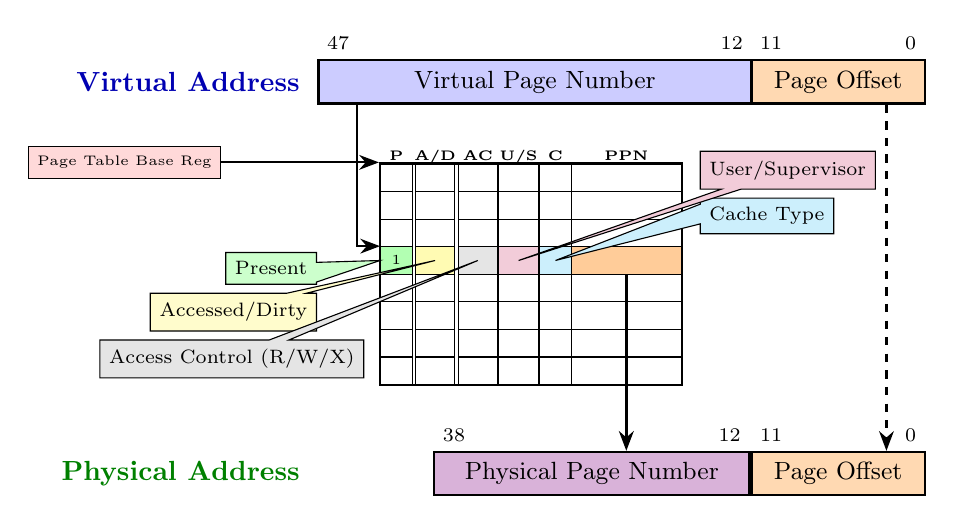
\begin{tikzpicture}[
    % Styles
    addrblock/.style={draw, thick, minimum height=0.55cm, font=\small},
    vpnblock/.style={addrblock, fill=blue!20},
    offsetblock/.style={addrblock, fill=orange!30},
    ppnblock/.style={addrblock, fill=violet!30},
    bitnumber/.style={font=\scriptsize},
    addrlabel/.style={font=\bfseries},
    ptecell/.style={draw, minimum height=0.38cm, font=\tiny, inner sep=1pt},
    arrowstyle/.style={-{Stealth[length=2.5mm]}, thick},
    callout/.style={font=\small},
]
    % Virtual Address bar
    \node[vpnblock, minimum width=5.5cm] (vpn) at (2.25, 2.8) {Virtual Page Number};
    \node[offsetblock, minimum width=2.2cm] (voffset) at (6.1, 2.8) {Page Offset};

    % Virtual Address title - left of VPN
    \node[addrlabel, blue!70!black, anchor=east] (vatitle) at ([xshift=-1mm]vpn.west) {Virtual Address};

    % Bit numbers for virtual address
    \node[bitnumber, anchor=south west] at (vpn.north west) {47};
    \node[bitnumber, anchor=south east] at (vpn.north east) {12};
    \node[bitnumber, anchor=south west] at (voffset.north west) {11};
    \node[bitnumber, anchor=south east] at (voffset.north east) {0};

    % Page Table using matrix of nodes
    \matrix[matrix of nodes,
            ampersand replacement=\&,
            column sep=-\pgflinewidth,
            row sep=-\pgflinewidth,
            nodes={draw, minimum height=0.35cm, font=\tiny, inner sep=1pt, anchor=center},
            column 1/.style={nodes={minimum width=0.4cm}},
            column 2/.style={nodes={minimum width=0.5cm}},
            column 3/.style={nodes={minimum width=0.5cm}},
            column 4/.style={nodes={minimum width=0.5cm}},
            column 5/.style={nodes={minimum width=0.4cm}},
            column 6/.style={nodes={minimum width=1.4cm}},
            row 1/.style={nodes={draw=none, font=\tiny\bfseries, minimum height=0.3cm, text depth=0pt, text height=0.2cm}},
            ] (pt) at (2.2, 0.5) {
        |[name=hdrP]| P \& A/D \& AC \& U/S \& C \& PPN \\
        |[name=r1c1]| \phantom{0} \& \phantom{0} \& \phantom{0} \& \phantom{0} \& \phantom{0} \& |[name=r1c6]| \phantom{0} \\
        \phantom{0} \& \phantom{0} \& \phantom{0} \& \phantom{0} \& \phantom{0} \& \phantom{0} \\
        \phantom{0} \& \phantom{0} \& \phantom{0} \& \phantom{0} \& \phantom{0} \& \phantom{0} \\
        |[fill=green!30, name=selP]| 1 \& |[fill=yellow!30, name=selAD]| \phantom{0} \& |[fill=gray!20, name=selAC]| \phantom{0} \& |[fill=purple!20, name=selUS]| \phantom{0} \& |[fill=cyan!20, name=selC]| \phantom{0} \& |[fill=orange!40, name=selPPN]| \phantom{0} \\
        \phantom{0} \& \phantom{0} \& \phantom{0} \& \phantom{0} \& \phantom{0} \& \phantom{0} \\
        \phantom{0} \& \phantom{0} \& \phantom{0} \& \phantom{0} \& \phantom{0} \& \phantom{0} \\
        \phantom{0} \& \phantom{0} \& \phantom{0} \& \phantom{0} \& \phantom{0} \& \phantom{0} \\
        |[name=rlastc1]| \phantom{0} \& \phantom{0} \& \phantom{0} \& \phantom{0} \& \phantom{0} \& |[name=rlastc6]| \phantom{0} \\
    };

    % Outer box around page table (excluding header)
    \node[draw, thick, inner sep=0pt, fit=(r1c1) (rlastc6)] (ptbox) {};

    % Page Table Base Register - positioned left of table north west
    \node[draw, fill=red!15, minimum height=0.4cm, font=\tiny,
          anchor=east] (ptbr) at ([xshift=-2cm]ptbox.north west) {Page Table Base Reg};

    % Arrow from PTBR to page table
    \draw[arrowstyle] (ptbr.east) -- (ptbox.north west);

    % Arrow from VPN to page table (index into table)
    \draw[arrowstyle] ([xshift=5mm]vpn.south west) |- (selP.north west);

    % Callouts for PTE fields - stacked on the left
    \node[rectangle callout, draw, fill=green!20, callout absolute pointer={(selP.west)},
        font=\scriptsize, anchor=east] (callP) at ([xshift=-8mm, yshift=-1mm]selP.west) {Present};
    \node[rectangle callout, draw, fill=yellow!20, callout absolute pointer={(selAD.center)},
        font=\scriptsize, anchor=north east] (callAD) at ([yshift=-1mm, xshift=0mm]callP.south east) {Accessed/Dirty};
    \node[rectangle callout, draw, fill=gray!20, callout absolute pointer={(selAC.center)},
        font=\scriptsize, anchor=north east] (callAC) at ([yshift=-1mm, xshift=6mm]callAD.south east) {Access Control (R/W/X)};
    \node[rectangle callout, draw, fill=cyan!20, callout absolute pointer={(selC.center)},
        font=\scriptsize, anchor=north west] (callC) at ([yshift=8mm, xshift=1mm]selC -| pt.east) {Cache Type};
    \node[rectangle callout, draw, fill=purple!20, callout absolute pointer={(selUS.center)},
        font=\scriptsize, anchor=south west] (callUS) at ([yshift=1mm]callC.north west) {User/Supervisor};

    % Physical Address bar
    \node[offsetblock, minimum width=2.2cm] (poffset) at ([yshift=-1cm]voffset |- pt.south) {Page Offset};
    \node[ppnblock, minimum width=4.0cm, anchor=east] (ppn) at (poffset.west) {Physical Page Number};

    % Physical Address title - x from vatitle, y from ppn
    \node[addrlabel, green!50!black, anchor=east] (patitle) at (vatitle.east |- ppn) {Physical Address};

    % Arrow from PTE physical page to physical address
    \draw[arrowstyle, line width=1.2pt] (selPPN.south) -- (selPPN |- ppn.north);

    % Bit numbers for physical address
    \node[bitnumber, anchor=south west] at (ppn.north west) {38};
    \node[bitnumber, anchor=south east] at (ppn.north east) {12};
    \node[bitnumber, anchor=south west] at (poffset.north west) {11};
    \node[bitnumber, anchor=south east] at (poffset.north east) {0};

    % Arrow showing page offset passes through
    \draw[arrowstyle, dashed] ([xshift=-5mm]voffset.south east) -- ([xshift=-5mm]poffset.north east);

\end{tikzpicture}
\end{center}
\vspace{-2mm}
\begin{columns}[T]
\column{0.5\textwidth}
\centering\footnotesize PTE -- Page Table Entry
\column{0.5\textwidth}
\centering\footnotesize Page size: $2^{12}$ bytes = 4KB
\end{columns}
\end{frame}

\begin{frame}{Page Table Location}
\begin{itemize}
\item Page table of each process resides in main memory; \textit{page table base register} points to entry 0
\item PTE address of virtual page \#VPN: \texttt{Page\_table\_base\_reg + VPN $\times$ PTE\_size}
\end{itemize}
\vspace{2mm}
\begin{center}
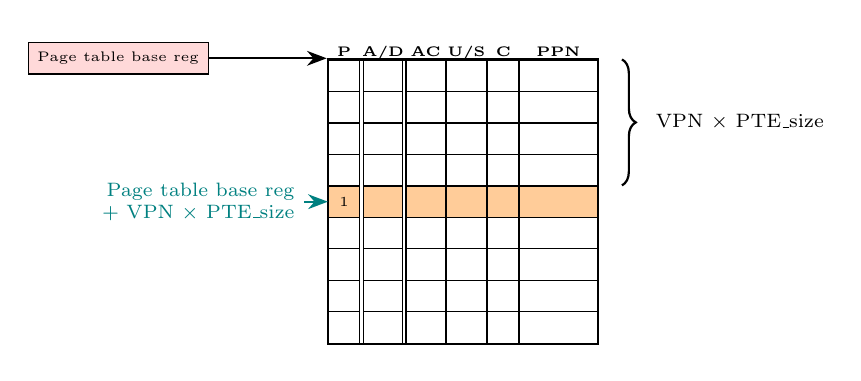
\begin{tikzpicture}[
    cell/.style={draw, minimum height=0.4cm, font=\tiny, inner sep=1pt, anchor=center},
    arrowstyle/.style={-{Stealth[length=2.5mm]}, thick},
]
    % Page Table using matrix of nodes
    \matrix[matrix of nodes,
            ampersand replacement=\&,
            column sep=-\pgflinewidth,
            row sep=-\pgflinewidth,
            nodes={cell},
            column 1/.style={nodes={minimum width=0.4cm}},
            column 2/.style={nodes={minimum width=0.5cm}},
            column 3/.style={nodes={minimum width=0.5cm}},
            column 4/.style={nodes={minimum width=0.5cm}},
            column 5/.style={nodes={minimum width=0.4cm}},
            column 6/.style={nodes={minimum width=1.0cm}},
            row 1/.style={nodes={draw=none, font=\tiny\bfseries, minimum height=0.3cm, text depth=0pt, text height=0.2cm}},
            ] (pt) at (0, 0) {
        P \& A/D \& AC \& U/S \& C \& PPN \\
        |[name=r1c1]| \phantom{0} \& \phantom{0} \& \phantom{0} \& \phantom{0} \& \phantom{0} \& |[name=r1c6]| \phantom{0} \\
        \phantom{0} \& \phantom{0} \& \phantom{0} \& \phantom{0} \& \phantom{0} \& \phantom{0} \\
        \phantom{0} \& \phantom{0} \& \phantom{0} \& \phantom{0} \& \phantom{0} \& \phantom{0} \\
        \phantom{0} \& \phantom{0} \& \phantom{0} \& \phantom{0} \& \phantom{0} \& \phantom{0} \\
        |[fill=orange!40, name=selRow]| 1 \& |[fill=orange!40]| \phantom{0} \& |[fill=orange!40]| \phantom{0} \& |[fill=orange!40]| \phantom{0} \& |[fill=orange!40]| \phantom{0} \& |[fill=orange!40, name=selEnd]| \phantom{0} \\
        \phantom{0} \& \phantom{0} \& \phantom{0} \& \phantom{0} \& \phantom{0} \& \phantom{0} \\
        \phantom{0} \& \phantom{0} \& \phantom{0} \& \phantom{0} \& \phantom{0} \& \phantom{0} \\
        \phantom{0} \& \phantom{0} \& \phantom{0} \& \phantom{0} \& \phantom{0} \& \phantom{0} \\
        |[name=rlastc1]| \phantom{0} \& \phantom{0} \& \phantom{0} \& \phantom{0} \& \phantom{0} \& |[name=rlastc6]| \phantom{0} \\
    };

    % Outer box around page table (excluding header)
    \node[draw, thick, inner sep=0pt, fit=(r1c1) (rlastc6)] (ptbox) {};

    % Page Table Base Register
    \node[draw, fill=red!15, minimum height=0.4cm, font=\tiny,
          anchor=east] (ptbr) at ([xshift=-1.5cm]ptbox.north west) {Page table base reg};

    % Arrow from PTBR to page table top
    \draw[arrowstyle] (ptbr.east) -- (ptbox.north west);

    % Label for base reg + VPN * PTE_size on left
    \node[font=\scriptsize, anchor=east, align=right, text=teal] (formula) at ([xshift=-3mm]selRow.west) {Page table base reg\\+ VPN $\times$ PTE\_size};
    \draw[arrowstyle, teal] (formula.east) -- (selRow.west);

    % VPN * PTE_size brace on right - from top of table content to highlighted row
    \draw[decorate, decoration={brace, amplitude=5pt}, thick]
        ([xshift=3mm]r1c6.north east) -- ([xshift=3mm]selEnd.north east)
        node[midway, xshift=3mm, font=\scriptsize, anchor=west] {VPN $\times$ PTE\_size};

\end{tikzpicture}
\end{center}
\end{frame}

\begin{frame}{Mapping Virtual Address Spaces to Physical Memory}
\begin{itemize}
\item Each process has its own page table; processes cannot access each other's memory (unless shared)
\item On context switch, Page Table Base Register is updated to the new process's table
\end{itemize}
\vspace{-2mm}
\begin{center}
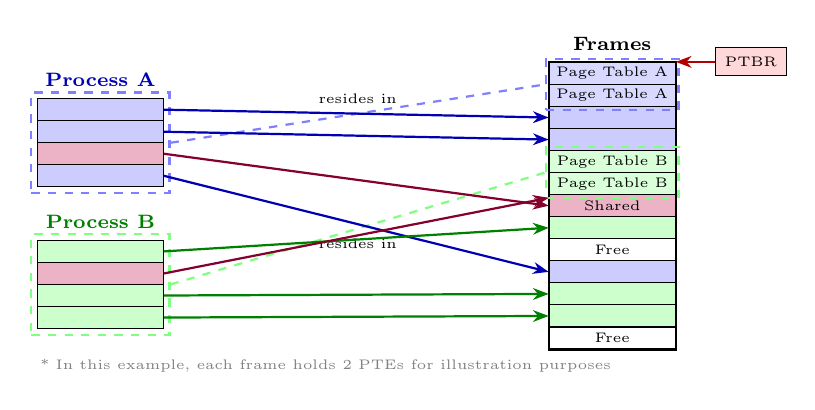
\begin{tikzpicture}[
    cell/.style={draw, minimum height=0.28cm, minimum width=1.6cm, font=\tiny, inner sep=0pt},
    arrowstyle/.style={-{Stealth[length=2mm]}, thick},
    mytitle/.style={font=\scriptsize\bfseries},
]
    % Process A Page Table (4 entries)
    \matrix[matrix of nodes,
            ampersand replacement=\&,
            column sep=-\pgflinewidth,
            row sep=-\pgflinewidth,
            nodes={cell},
            ] (ptA) at (-2.5, 0.3) {
        |[fill=blue!20, name=ptA1]| \phantom{0} \\
        |[fill=blue!20, name=ptA2]| \phantom{0} \\
        |[fill=purple!30, name=ptA3]| \phantom{0} \\
        |[fill=blue!20, name=ptA4]| \phantom{0} \\
    };
    \node[mytitle, blue!70!black, anchor=south, yshift=-1mm] at (ptA.north) {Process A};
    \node[draw, thick, dashed, blue!50, inner sep=2pt, fit=(ptA1) (ptA4)] (ptAbox) {};


    % Process B Page Table (4 entries)
    \matrix[matrix of nodes,
            ampersand replacement=\&,
            column sep=-\pgflinewidth,
            row sep=-\pgflinewidth,
            nodes={cell},
            ] (ptB) at (-2.5, -1.5) {
        |[fill=green!20, name=ptB1]| \phantom{0} \\
        |[fill=purple!30, name=ptB2]| \phantom{0} \\
        |[fill=green!20, name=ptB3]| \phantom{0} \\
        |[fill=green!20, name=ptB4]| \phantom{0} \\
    };
    \node[mytitle, green!50!black, anchor=south, yshift=-1mm] at (ptB.north) {Process B};
    \node[draw, thick, dashed, green!50, inner sep=2pt, fit=(ptB1) (ptB4)] (ptBbox) {};


    % Physical Frames - page tables are contiguous in memory
    \matrix[matrix of nodes,
            ampersand replacement=\&,
            column sep=-\pgflinewidth,
            row sep=-\pgflinewidth,
            nodes={cell},
            ] (frames) at (4, -0.5) {
        |[fill=blue!15, name=f0]| Page Table A \\
        |[fill=blue!15, name=f1]| Page Table A \\
        |[fill=blue!20, name=f2]| \phantom{0} \\
        |[fill=blue!20, name=f3]| \phantom{0} \\
        |[fill=green!15, name=f4]| Page Table B \\
        |[fill=green!15, name=f5]| Page Table B \\
        |[fill=purple!30, name=f6]| Shared \\
        |[fill=green!20, name=f7]| \phantom{0} \\
        |[name=f8]| Free \\
        |[fill=blue!20, name=f9]| \phantom{0} \\
        |[fill=green!20, name=f10]| \phantom{0} \\
        |[fill=green!20, name=f11]| \phantom{0} \\
        |[name=f12]| Free \\
    };
    \node[mytitle, anchor=south, yshift=-1mm] at (frames.north) {Frames};
    \node[draw, thick, inner sep=0pt, fit=(f0) (f12)] (framesbox) {};

    % Dashed borders around Page Table frames in physical memory
    \node[draw, thick, dashed, blue!50, inner sep=1pt, fit=(f0) (f1)] (ptAphys) {};
    \node[draw, thick, dashed, green!50, inner sep=1pt, fit=(f4) (f5)] (ptBphys) {};

    % Dashed lines from page table boxes to contiguous Page Table frames
    \draw[dashed, thick, blue!50] (ptAbox.east) -- (ptAphys.west)
        node[midway, above, font=\tiny, text=black] {resides in};
    \draw[dashed, thick, green!50] (ptBbox.east) -- (ptBphys.west)
        node[midway, below, font=\tiny, text=black] {resides in};

    % Straight arrows from Process A PTEs to data frames
    \draw[arrowstyle, blue!70!black] (ptA1.east) -- (f2.west);
    \draw[arrowstyle, blue!70!black] (ptA2.east) -- (f3.west);
    \draw[arrowstyle, blue!70!black] (ptA4.east) -- (f9.west);
    \draw[arrowstyle, purple!70!black] (ptA3.east) -- (f6.west);

    % Straight arrows from Process B PTEs to data frames
    \draw[arrowstyle, green!50!black] (ptB1.east) -- (f7.west);
    \draw[arrowstyle, green!50!black] (ptB3.east) -- (f10.west);
    \draw[arrowstyle, green!50!black] (ptB4.east) -- (f11.west);
    \draw[arrowstyle, purple!70!black] (ptB2.east) -- ([yshift=1mm]f6.west);

    % PTBR - right of frames, pointing to Page Table A in physical memory
    \node[draw, fill=red!15, font=\tiny, minimum height=0.28cm, anchor=west] (ptbr) at ([xshift=5mm]f0.north east) {PTBR};
    \draw[arrowstyle, red!70!black] (ptbr.west) -- (f0.north east);

    % Note about illustration simplification
    \node[font=\tiny, text=gray, anchor=north west] at (ptBbox.south west |- f12.south)
        {* In this example, each frame holds 2 PTEs for illustration purposes};

\end{tikzpicture}
\end{center}
\end{frame}

\begin{frame}[fragile]{Page Fault}
\begin{columns}[T]
\column{0.45\textwidth}
\textbf{Present bit = 0} $\rightarrow$ page not in memory
\begin{itemize}
\item CPU traps to OS (cannot handle itself)
\item OS loads page from disk, updates PTE
\item CPU retries the access
\end{itemize}
\column{0.55\textwidth}
\begin{lstlisting}[style=pseudocode, basicstyle=\ttfamily\scriptsize]
// OS: Present bit = 0
handle_non_present_page(vaddr):
  vpn = vaddr >> PAGE_BITS

  if no_free_physical_page():
    victim = select_victim()  // LRU, etc.
    if victim.dirty:
      write_to_swap(victim)
    victim.pte.present = 0

  ppn = allocate_physical_page()
  read_from_disk(vpn, ppn)

  pte[vpn].ppn = ppn
  pte[vpn].present = 1
  return_to_user()  // retry access
\end{lstlisting}
\end{columns}
\end{frame}

\begin{frame}[fragile]{Protection Violation Fault}
\begin{columns}[T]
\column{0.45\textwidth}
\textbf{Access control bits}: R~(read), W~(write), X~(execute)
\begin{itemize}
\item CPU checks permissions on every access
\item Violation $\rightarrow$ trap to OS
\item \textbf{Not always a crash!}
    \begin{itemize}
    \item Copy-on-Write (COW)
    \item Dirty bit emulation
    \item Guard pages (stack growth)
    \end{itemize}
\end{itemize}
\column{0.55\textwidth}
\begin{lstlisting}[style=pseudocode, basicstyle=\ttfamily\scriptsize]
// OS: Access control violation
handle_protection_violation(vaddr, access):
  vpn = vaddr >> PAGE_BITS

  // Copy-on-Write: shared page,
  // write triggers private copy
  if is_cow_page(vpn) && access == WRITE:
    new_ppn = copy_page(pte[vpn].ppn)
    pte[vpn].ppn = new_ppn
    pte[vpn].writable = 1
    return_to_user()  // retry

  // Dirty tracking for swapping
  if tracking_dirty(vpn) && access == WRITE:
    pte[vpn].dirty = 1
    pte[vpn].writable = 1
    return_to_user()

  kill_process(SIGSEGV)  // real violation
\end{lstlisting}
\end{columns}
\end{frame}

\begin{frame}{Optimal Page Size}
\begin{itemize}
\item \textbf{Minimize wasted storage}
    \begin{itemize}
    \item Small pages minimize internal fragmentation
    \item Small pages increase the size of the page tables
    \end{itemize}
\item \textbf{Minimize transfer time – use large pages (multiple disk sectors)}
    \begin{itemize}
    \item Amortize access cost and prefetch useful data
    \item But, might transfer unnecessary data and discard (victimize) useful data
    \end{itemize}
\item \textbf{General trend toward larger pages because}
    \begin{itemize}
    \item Big cheap RAM
    \item Increasing memory / disk performance gap
    \item Larger address spaces
    \item Programs with larger code and data
    \end{itemize}
\end{itemize}
\end{frame}

\section{TLB and Cache Design}

\begin{frame}{Translation Look aside Buffer (TLB)}
\begin{itemize}
\item With virtual memory, before each cache access, need to first get the physical address
    \begin{itemize}
    \item The page table resides in memory $\rightarrow$ each translation requires an extra memory access
    \end{itemize}
\item The TLB is a cache for recent address translations
\end{itemize}
\begin{center}
[Diagram: TLB caching page table entries]
\end{center}
\end{frame}


\begin{frame}{Translation Look aside Buffer (TLB)}
\begin{columns}[T]
\begin{column}{0.57\textwidth}
\begin{itemize}
\item \textbf{The TLB caches recently used PTEs}
\item[] Typically, 128--256 entries, 4--8 ways
    
\item \textbf{TLB Indexing}

\begin{center}
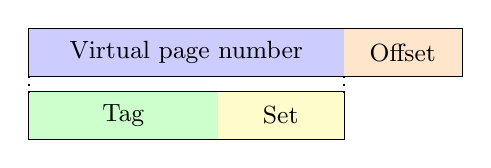
\begin{tikzpicture}[scale=1]
    % Virtual address breakdown
    \draw[thick] (0,0) rectangle (5.5,0.6);
    \draw[thick] (4,0) -- (4,0.6);
    
    % Fill colors
    \fill[blue!20] (0,0) rectangle (4,0.6);
    \fill[orange!20] (4,0) rectangle (5.5,0.6);
    
    % Labels
    \node at (2,0.3) {\small Virtual page number};
    \node at (4.75,0.3) {\small Offset};
    
    % Tag and Set subdivision
    \draw[thick] (0,-0.8) rectangle (4,-0.2);
    \draw[thick] (2.4,-0.8) -- (2.4,-0.2);
    
    \fill[green!20] (0,-0.8) rectangle (2.4,-0.2);
    \fill[yellow!20] (2.4,-0.8) rectangle (4,-0.2);
    
    \node at (1.2,-0.5) {\small Tag};
    \node at (3.2,-0.5) {\small Set};
    
    % Dotted lines connecting
    \draw[dotted, thick] (0,0) -- (0,-0.2);
    \draw[dotted, thick] (4,0) -- (4,-0.2);
\end{tikzpicture}
\end{center}

\item \textbf{On A TLB miss}
    \begin{itemize}
    \item Page Miss Handler (PMH) loads address PTBR+VPN$\times$PTE\_size to read PTE
    \item PMH may contain a 2\textsuperscript{nd} level TLB
    \end{itemize}
    
\item \textbf{OS maintains TLB coherency}
\item[] OS updates PTE $\rightarrow$ OS must invalidate PTE in TLB
\end{itemize}
\end{column}

\begin{column}{0.43\textwidth}
\begin{center}
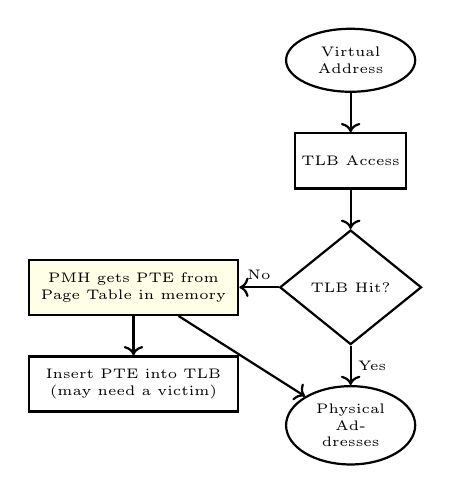
\begin{tikzpicture}[
    node distance=5mm,
    box/.style={rectangle, draw, thick, minimum width=1cm, minimum height=0.7cm, text centered, font=\tiny},
    decision/.style={diamond, draw, thick, minimum width=1.8cm, minimum height=1cm, text centered, font=\tiny},
    oval/.style={ellipse, draw, thick, minimum width=1cm, minimum height=0.8cm, text centered, font=\tiny, text width=1cm},
    arrow/.style={->, thick}]
    \tiny
    % Nodes
    \node[oval, align=center] (va) {Virtual Address};
    \node[box, align=center, below=of va] (tlb) {TLB Access};
    \node[decision, below=of tlb] (hit) {TLB Hit?};
    \node[box, fill=yellow!10, align=center, left=of hit, text width=2.5cm] (pmh) {PMH gets PTE from Page Table in memory};
    \node[box, align=center, below=of pmh, text width=2.5cm] (insert) {Insert PTE into TLB (may need a victim)};
    \node[oval, align=center, below=of hit] (pa) {Physical Addresses};
    
    % Arrows
    \draw[arrow] (va) -- (tlb);
    \draw[arrow] (tlb) -- (hit);
    \draw[arrow] (hit) -- node[above] {No} (pmh);
    \draw[arrow] (hit) -- node[right] {Yes} (pa);
    \draw[arrow] (pmh) -- (insert);
    \draw[arrow] (pmh) -- (pa);
    
\end{tikzpicture}
\end{center}
\end{column}
\end{columns}
\end{frame}

\begin{frame}{Processor Caches and TLBs}
\begin{itemize}
\item Each of L1 I\$ and L1 D\$ has its own TLB – ITLB and DTLB
    \begin{itemize}
    \item Similar to the I\$ and the D\$, the ITLB and DTLB are accessed in different pipe-stages
    \end{itemize}
\item In case of either ITLB or DTLB miss: access the STLB (second level TLB)
\item In case of STLB miss
    \begin{itemize}
    \item PMH (page miss handler) injects a load to get the PTE from the page table (page walk)
    \item This load, like any other load, starts by a lookup in the L1 D\$
    \end{itemize}
\end{itemize}
\begin{center}
[Diagram: Core with L1 I\$, L1 D\$, ITLB, DTLB, STLB, L2, L3, and Memory hierarchy]
\end{center}
\end{frame}

\begin{frame}{Virtual Memory and Cache}
\centering
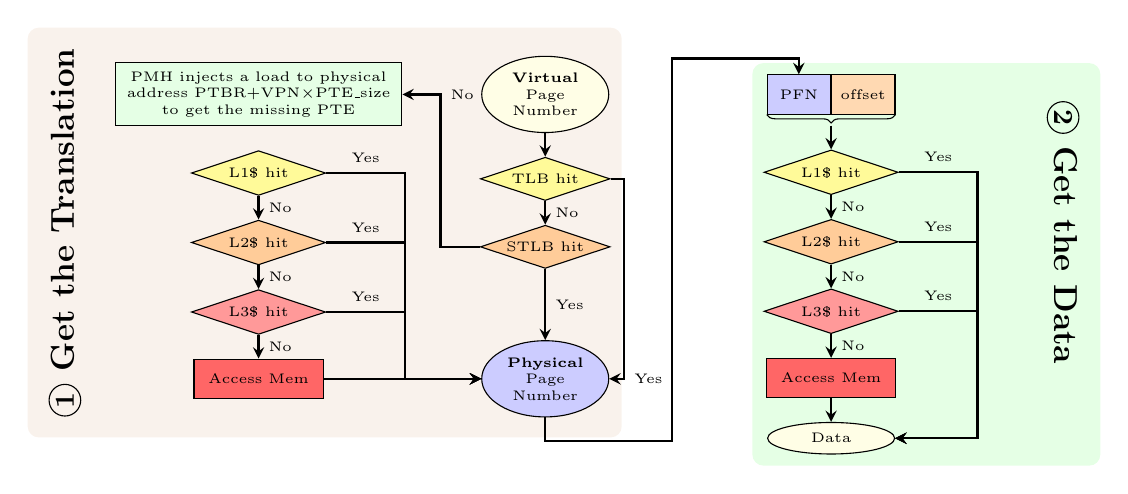
\begin{tikzpicture}[
    node distance=3mm,
    decision/.style={diamond, draw, fill=blue!10, text width=1cm, align=center, inner sep=1pt, minimum height=0.3cm, aspect=3, font=\tiny},
    process/.style={rectangle, draw, fill=green!10, text width=1.5cm, align=center, minimum height=0.5cm, inner sep=2pt, font=\tiny},
    data/.style={ellipse, draw, fill=yellow!10, text width=1cm, align=center, minimum height=0.4cm, inner sep=2pt, font=\tiny},
    l1hit/.style={decision, fill=yellow!40},
    l2hit/.style={decision, fill=orange!40},
    l3hit/.style={decision, fill=red!40},
    accessmem/.style={process, fill=red!60},
    arrow/.style={->, >=stealth, thick},
    every node/.style={font=\tiny}
]

% Top section - TLB lookup
\node[data] (vpn) {\textbf{Virtual} Page Number};
\node[l1hit, below=of vpn] (tlb) {TLB hit};
\node[l2hit, below=of tlb] (stlb) {STLB hit};

% Translation path
\node[process, left=1cm of vpn, text width=3.5cm, minimum height=0.8cm] (pmh) {PMH injects a load to physical address PTBR+VPN$\times$PTE\_size to get the missing PTE};
%\node[process, below=of pmh] (trans) {Get the Translation};
\node[l1hit, below=of pmh] (l1) {L1\$ hit};
\node[l2hit, below=of l1] (l2) {L2\$ hit};
\node[l3hit, below=of l2] (l3) {L3\$ hit};
\node[accessmem, below=of l3] (mem1) {Access Mem};

\node[data, fill=blue!20] (pfn) at (mem1 -| stlb) {\textbf{Physical} Page Number};


% Data path
\node[rectangle, draw, fill=blue!20, minimum width=0.8cm, minimum height=0.5cm, font=\tiny, right=2cm of vpn] (pfnbox) {PFN};
\node[rectangle, draw, fill=orange!30, minimum width=0.8cm, minimum height=0.5cm, font=\tiny, right=0pt of pfnbox] (offsetbox) {offset};
\draw[decorate, decoration={brace, mirror, amplitude=3pt}] (pfnbox.south west) -- (offsetbox.south east) coordinate[midway, below=4pt] (bracepoint);
\node[l1hit, below=of bracepoint] (l1d) {L1\$ hit};
\node[l2hit, below=of l1d] (l2d) {L2\$ hit};
\node[l3hit, below=of l2d] (l3d) {L3\$ hit};
\node[accessmem, below=of l3d] (mem2) {Access Mem};
\node[data, below=of mem2] (data) {Data};

% Arrows
\draw[arrow] (vpn) -- (tlb);
\draw[arrow] (tlb) -- node[right] {No} (stlb);
\draw[arrow] (tlb) -- ++(1,0) |- node[right] {Yes} (pfn);
\draw[arrow] (stlb.west) -- ++(-0.5, 0) |- node[right] {No} (pmh.east);
\draw[arrow] (stlb.south) -- node[right] {Yes} (pfn);
%\draw[arrow] (pmh) -- (l1);
\draw[arrow] (l1) -- node[right] {No} (l2);
\draw[arrow] (l2) -- node[right] {No} (l3);
\draw[arrow] (l3) -- node[right] {No} (mem1);
\draw[arrow] (l1.east) -- node[above] {Yes} ++(1,0) |- (pfn);
\draw[arrow] (l2.east) -- node[above] {Yes} ++(1,0) |- (pfn);
\draw[arrow] (l3.east) -- node[above] {Yes} ++(1,0) |- (pfn);
\draw[arrow] (mem1) -- (pfn);
%\draw[arrow] (pmh) |- (getdata);
\draw[arrow] (pfn.south) -- ++(0, -0.3) -| ($(pfn)!0.5!(pfnbox)$) |- ([yshift=2mm]pfnbox.north) -- (pfnbox.north);
\draw[arrow] (bracepoint) -- (l1d);
\draw[arrow] (l1d) -- node[right] {No} (l2d);
\draw[arrow] (l2d) -- node[right] {No} (l3d);
\draw[arrow] (l3d) -- node[right] {No} (mem2);
\draw[arrow] (l1d.east) -- node[above] {Yes} ++(1,0) |- (data);
\draw[arrow] (l2d.east) -- node[above] {Yes} ++(1,0) |- (data);
\draw[arrow] (l3d.east) -- node[above] {Yes} ++(1,0) |- (data);
\draw[arrow] (mem2.south) -- (data);

% Rotated labels (defined first so they can be included in fit)
\node[rotate=90, font=\large\bfseries, above left=3mm and 3mm of pmh] (translabel) {\tikz[baseline=(c.base)]{\node[circle, draw, inner sep=1pt, font=\normalsize\bfseries] (c) {1};} Get the Translation};
\coordinate (dataright) at ([xshift=18mm]data.east);
\node[rotate=-90, font=\large\bfseries, anchor=south] at (dataright |- translabel) (datalabel) {\tikz[baseline=(c.base)]{\node[circle, draw, inner sep=1pt, font=\normalsize\bfseries] (c) {2};} Get the Data};

% Background for sections (including labels)
\begin{scope}[on background layer]
\node[fit=(pmh)(vpn)(tlb)(stlb)(l1)(l2)(l3)(mem1)(pfn)(translabel), fill=brown!10, rounded corners, inner sep=4pt] (transbg) {};
\node[fit=(pfnbox)(offsetbox)(l1d)(l2d)(l3d)(mem2)(data)(datalabel), fill=green!10, rounded corners, inner sep=4pt] (databg) {};
\end{scope}

\end{tikzpicture}

\vspace{-2mm}
\footnotesize
\begin{itemize}
\item Page table entries are cached in L1 D\$, L2\$ and L3\$ as data
\item Cache miss on injected load $\Rightarrow$ cache line fill brings all PTEs in that line into cache
\item Only the specific missed PTE is filled into the STLB and TLB
\end{itemize}
\end{frame}


\begin{frame}{Overlapping TLB \& Cache Access}
\begin{columns}[T]
\column{0.38\textwidth}
\textbf{Goal:} Start cache access in parallel to TLB access
\begin{itemize}
    \item Save a cycle on TLB hit + cache hit
\end{itemize}

\textbf{Cache \#set contained in page offset}
\begin{itemize}
    \item Cache set available before translation
    \item Access cache set in parallel with TLB
    \item Once translation done, match physical page\# with tag of each way
\end{itemize}

\textbf{Restriction on cache:}
\begin{itemize}
    \item \#sets $\times$ line size = way size $\leq$ page size
    \item Cache size $\leq$ page size $\times$ associativity
\end{itemize}

\column{0.62\textwidth}
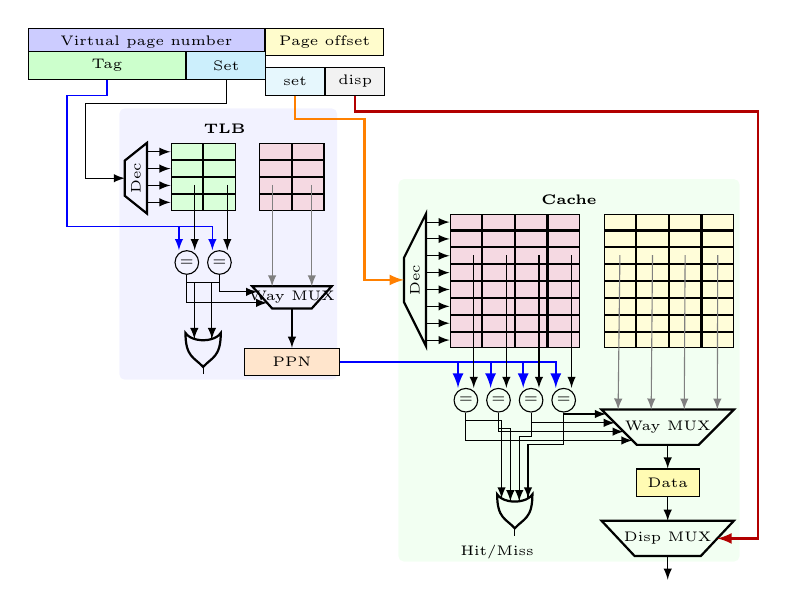
\begin{tikzpicture}[
    node distance=5mm,
    addr/.style={draw, rectangle, minimum height=0.35cm, inner sep=1pt, font=\tiny},
    tlbcell/.style={draw, minimum width=4mm, minimum height=2mm, inner sep=0pt, font=\tiny},
    cachecell/.style={draw, minimum width=4mm, minimum height=2mm, inner sep=0pt, font=\tiny},
    comp/.style={circle, draw, inner sep=0pt, minimum size=3mm, font=\tiny},
    label/.style={font=\tiny\bfseries},
    arrow/.style={->, >=latex},
    bgbox/.style={draw=none, rounded corners=2pt, inner sep=2pt}
]

% Virtual Address at top - using current page as reference
\node[addr, fill=blue!20, minimum width=3cm] (vpn) at (current page.center) {Virtual page number};
\node[addr, fill=yellow!20, minimum width=1.5cm, right=0pt of vpn] (poffset) {Page offset};

% Tag and Set below VPN
\node[addr, fill=green!20, minimum width=2cm, below=3mm of vpn.west, anchor=west] (vtag) {Tag};
\node[addr, fill=cyan!20, minimum width=1cm, right=0pt of vtag] (vset) {Set};

% Set# and disp below page offset - as a breakdown of page offset (slightly lower)
\node[addr, fill=cyan!10, minimum width=0.75cm, below=5mm of poffset.west, anchor=west] (pset) {set};
\node[addr, fill=gray!10, minimum width=0.75cm, right=0pt of pset] (pdisp) {disp};

% TLB Structure
% TLB Set decoder - positioned below vset
\node[muxdemux, muxdemux def={NB=0, NT=1, NR=4, NL=1, Lh=0.8, Rh=1.6, w=0.5},
        external pins width=0, below left=8mm and 5mm of vset, font=\tiny] 
    (tlbdec) {\rotatebox{90}{Dec}};

% TLB Tag array (4 sets x 2 ways) - relative to decoder right pins
\node[tlbcell, fill=green!15, right=3mm of tlbdec.rpin 1] (tlbtag-0-0) {};
\foreach \way in {1,...,1} {
    \node[tlbcell, fill=green!15, right=0pt of tlbtag-0-\the\numexpr\way-1\relax] (tlbtag-0-\way) {};
}
\foreach \set in {1,...,3} {
    \foreach \way in {0,...,1} {
        \node[tlbcell, fill=green!15, below=0pt of tlbtag-\the\numexpr\set-1\relax-\way] (tlbtag-\set-\way) {};
    }
}

% TLB Value array - relative to tag array
\node[tlbcell, fill=purple!15, right=3mm of tlbtag-0-1] (tlbval-0-0) {};
\foreach \way in {1,...,1} {
    \node[tlbcell, fill=purple!15, right=0pt of tlbval-0-\the\numexpr\way-1\relax] (tlbval-0-\way) {};
}
\foreach \set in {1,...,3} {
    \foreach \way in {0,...,1} {
        \node[tlbcell, fill=purple!15, below=0pt of tlbval-\the\numexpr\set-1\relax-\way] (tlbval-\set-\way) {};
    }
}

% TLB comparators below tags - aligned with tag outputs
\node[comp, anchor=north, below=of tlbtag-3-0.south] (tlbcomp-0) {=};
\foreach \way in {1,...,1} {
    \node[comp, anchor=north, below=of tlbtag-3-\way.south] (tlbcomp-\way) {=};
}

% OR gate for TLB hit/miss - centered between comparators
\coordinate (tlb-or-x) at ($(tlbcomp-0.south)!0.5!(tlbcomp-1.south)$);
\node[or port, scale=0.4, number inputs=2, rotate=-90, external pins width=0] (tlbor) at ([yshift=-12mm]tlb-or-x) {};

% TLB Way MUX - positioned to match width of value table (2 ways)
\node[muxdemux, muxdemux def={NT=2, NB=1, NL=1, NR=2, Lh=0.9, Rh=1.8, w=0.5}, external pins width=0, rotate=90] 
    (tlbmux) at ([yshift=-11mm]tlbval-3-0.south east) {};
\node[font=\tiny, align=center] at (tlbmux) {Way MUX};

% Physical page# output - below mux
\node[addr, fill=orange!20, minimum width=1.2cm, below=of tlbmux.blpin 1] (ppn) {PPN};

% Cache Structure
% Cache Set decoder - positioned below pset
\node[muxdemux, muxdemux def={NB=0, NT=1, NR=8, NL=1, Lh=1, Rh=3, w=0.5},
        external pins width=0, below right=15mm and 10mm of pset, font=\tiny]
        (cachedec) {\rotatebox{90}{Dec}};

% Cache Tag array - relative to decoder right pins
\node[cachecell, fill=purple!15, right=3mm of cachedec.rpin 1] (ctag-0-0) {};
\foreach \way in {1,...,3} {
    \node[cachecell, fill=purple!15, right=0pt of ctag-0-\the\numexpr\way-1\relax] (ctag-0-\way) {};
}
\foreach \set in {1,...,7} {
    \foreach \way in {0,...,3} {
        \node[cachecell, fill=purple!15, below=0pt of ctag-\the\numexpr\set-1\relax-\way] (ctag-\set-\way) {};
    }
}

% Cache Data array - relative to tag array
\node[cachecell, fill=yellow!15, right=3mm of ctag-0-3] (cdata-0-0) {};
\foreach \way in {1,...,3} {
    \node[cachecell, fill=yellow!15, right=0pt of cdata-0-\the\numexpr\way-1\relax] (cdata-0-\way) {};
}
\foreach \set in {1,...,7} {
    \foreach \way in {0,...,3} {
        \node[cachecell, fill=yellow!15, below=0pt of cdata-\the\numexpr\set-1\relax-\way] (cdata-\set-\way) {};
    }
}

% Cache comparators below tags - aligned with tag outputs
\node[comp, anchor=north, below=of ctag-7-0.south] (ccomp-0) {=};
\foreach \way in {1,...,3} {
    \node[comp, anchor=north, below=of ctag-7-\way.south] (ccomp-\way) {=};
}

% OR gate for cache hit/miss - centered between leftmost and rightmost comparators
\coordinate (cache-or-x) at ($(ccomp-0.south)!0.5!(ccomp-3.south)$);
\node[or port, scale=0.4, number inputs=4, rotate=-90, external pins width=0] (cacheor) at ([yshift=-15mm]cache-or-x) {};

% Cache Way MUX - positioned to match width of data table (4 ways)
\node[muxdemux, muxdemux def={NT=4, NB=1, NL=1, NR=4, Lh=1.4, Rh=3, w=0.8}, external pins width=0, rotate=90] 
    (cachemux) at ([yshift=-10mm, xshift=4mm]cdata-7-1.south west) {};
\node[font=\tiny, align=center] at (cachemux) {Way MUX};

% Hit/Miss output - relative to OR gate
\node[font=\tiny, below=3mm of cacheor, align=center] {Hit/Miss};

% Data output - below mux
\node[addr, fill=yellow!30, minimum width=0.8cm, below=3mm of cachemux.blpin 1] (dataout) {Data};

% Displacement MUX - below data, with narrow part at bottom
\node[muxdemux, muxdemux def={NT=2, NB=1, NL=1, NR=1, Lh=1.5, Rh=3, w=0.8}, rotate=90, external pins width=0, below=3mm of dataout, anchor=brpin 1, font=\tiny] 
    (dispmux) {\rotatebox{-90}{Disp MUX}};

% Add labels centered between decoder and arrays
\coordinate (tlb-label-x) at ($(tlbdec.west)!0.5!(tlbval-0-1.east)$);
\node[label] (tlblabel) at (tlb-label-x |- tlbdec.north) [above=0mm] {TLB};

\coordinate (cache-label-x) at ($(cachedec.west)!0.5!(cdata-0-3.east)$);
\node[label] (cachelabel) at (cache-label-x |- cachedec.north) [above=0mm] {Cache};

% Add colored backgrounds using fit
% TLB background
\begin{scope}[on background layer]
    \node[bgbox, fill=blue!5, fit=(tlblabel)(tlbdec)(tlbtag-0-0)(tlbval-3-1)(tlbcomp-0)(tlbcomp-1)(tlbor)(tlbmux)] (tlbbg) {};
\end{scope}

% Cache background
\begin{scope}[on background layer]
    \node[bgbox, fill=green!5, fit=(cachelabel)(cachedec)(ctag-0-0)(cdata-7-3)(ccomp-0)(ccomp-3)(cacheor)(cachemux)(dispmux)] (cachebg) {};
\end{scope}

% Connections
% VPN set to TLB decoder (from left side)
\draw[arrow] (vset.south) -- ++(0,-0.3) -|  ([xshift=-5mm]tlbdec.blpin 1) -- (tlbdec.blpin 1);

% Tag from address to all TLB comparators (from top with slight offset)
\foreach \way in {0,...,1} {
    \draw[arrow, blue] (vtag.south) 
        |- ([xshift=5mm, yshift=-2mm] vtag.south west)
        |- ([xshift={-1mm + 0.3*\way}, yshift=3mm]tlbcomp-\way.north)
        -- ([xshift={-1mm + 0.3*\way}]tlbcomp-\way.north);
}

% Page offset set to Cache (from left side - highlighted in orange)
\draw[arrow, orange, thick] (pset.south) -- ++(0,-0.3) -| ([xshift=-5mm]cachedec.blpin 1) -- (cachedec.blpin 1);

% Decoder outputs to TLB array rows
\foreach \set in {0,...,3} {
    \draw[arrow] (tlbdec.brpin \the\numexpr\set+1\relax |- tlbtag-\set-0.west) -- (tlbtag-\set-0.west);
}

% Decoder outputs to Cache array rows
\foreach \set in {0,...,7} {
    \draw[arrow] (cachedec.brpin \the\numexpr\set+1\relax |- ctag-\set-0.west) -- (ctag-\set-0.west);
}

% Selected TLB row output to comparators (from top with slight offset)
\foreach \way in {0,...,1} {
    \draw[arrow] ([xshift=1mm, yshift=-1mm]tlbtag-1-\way.south -| tlbcomp-\way.north) -- ([xshift=1mm]tlbcomp-\way.north);
}

% Comparator outputs to OR gate for hit detection
\foreach \way in {0,...,1} {
    \pgfmathtruncatemacro{\inputnum}{1 + \way}
    \draw[arrow] (tlbcomp-\way.south) -- ++(0,-0.1) -| (tlbor.bin \inputnum);
    \draw[arrow] (tlbcomp-\way.south) |- (tlbmux.btpin \inputnum);
}

% TLB values to mux - from same row as tag outputs, straight down
\foreach \way in {0,...,1} {
    \pgfmathtruncatemacro{\muxpin}{2 - \way}
    \draw[arrow, gray] ([yshift=-1mm]tlbval-1-\way.south -| tlbmux.brpin \muxpin) -- (tlbmux.brpin \muxpin);
}

% TLB mux output to physical page#
\draw[arrow] (tlbmux.blpin 1) -- (ppn.north);

% Physical page# to all cache comparators (from top with slight offset)
\foreach \way in {0,...,3} {
    \draw[arrow, blue, thick] (ppn.east) -| ([xshift={-1mm}]ccomp-\way.north);
}

% Selected cache row to comparators (consistent with TLB style)
\foreach \way in {0,...,3} {
    \draw[arrow] ([xshift=1mm, yshift=-1mm]ctag-1-\way.south -| ccomp-\way.north) -- ([xshift=1mm]ccomp-\way.north);
}

% Cache comparator outputs to OR gate for hit detection (staggered to avoid overlaps)
\foreach \way in {0,...,3} {
    \pgfmathtruncatemacro{\inputnum}{4 - \way}
    \pgfmathsetmacro{\yoffset}{-1 - \way}  % Start at -3mm, each subsequent 1mm lower
    \draw[arrow] (ccomp-\way.south) -- ++(0,\yoffset mm) -| (cacheor.bin \inputnum);
}

% Cache comparator outputs to displacement MUX control
\foreach \way in {0,...,3} {
    \pgfmathtruncatemacro{\inputnum}{1 + \way}
    \draw[arrow] (ccomp-\way.south) |- (cachemux.btpin \inputnum);
}

% Cache data to mux - from same row as tag outputs, straight down
\foreach \way in {0,...,3} {
    \pgfmathtruncatemacro{\muxpin}{\way + 1}
    \draw[arrow, gray] ([yshift=-1mm]cdata-1-\way.south) -- (cachemux.brpin \muxpin);
}

% Mux output to data output
\draw[arrow] (cachemux.blpin 1) -- (dataout.north);

% Data to displacement MUX (top input)
\draw[arrow] (dataout.south) -- (dispmux.brpin 1);

% Disp signal from pdisp to displacement MUX control (routed from right of cache data table)
\draw[arrow, red!70!black, thick] (pdisp.south) 
    |- ([xshift=3mm, yshift=-2mm]pdisp.south -| cdata-7-3.east)
    -- ([xshift=3mm]cdata-7-3.south east) 
    |- (dispmux.bbpin 1);

% Displacement MUX output to final output
\draw[arrow] (dispmux.blpin 1) -- ++(0, -0.3);
\end{tikzpicture}
\end{columns}
\end{frame}


\begin{frame}{Overlapping TLB \& Cache Access}
\textbf{Goal:} start cache access in parallel to TLB access
\begin{itemize}
\item Save a cycle on getting the data in case of TLB hit and cache hit
\end{itemize}

\textbf{Cache \#set contained in page offset}
\begin{itemize}
\item Cache set available before translation
\item Access cache set in parallel with TLB
\item Once translation is done, match physical page number with tag of each way
\end{itemize}

\textbf{Restriction on cache}
\begin{itemize}
\item \#sets $\times$ line size = way size $\leq$ page size
\item Cache size $\leq$ page size $\times$ associativity
\end{itemize}
\end{frame}

\begin{frame}[fragile]{Evicting a Page to Disk}
\begin{columns}[T]
\column{0.42\textwidth}
\textbf{OS updates the Page Table}
\begin{itemize}
\item Invalidate page from TLBs: invalidate on all cores
\item Mark page as not present in PTE
\item MESI keeps cached PTEs coherent
\item Store disk location in PTE
\end{itemize}

\textbf{OS copies page to disk}
\begin{itemize}
\item Only if dirty bit set (page modified)
\item Clean pages: just discard
\end{itemize}
\column{0.58\textwidth}
\begin{lstlisting}[style=pseudocode, basicstyle=\ttfamily\scriptsize]
// OS: Evict page to make room
evict_page_to_disk(victim_vpn):
  // 1. TLB shootdown (all cores)
  tlb_shootdown(victim_vpn)  // IPI to other cores

  // 2. Update page table
  pte[victim_vpn].present = 0

  // 3. Write to disk only if dirty
  if pte[victim_vpn].dirty:
    disk_loc = find_swap_slot()
    pte[victim_vpn].disk_loc = disk_loc
    paddr = victim_ppn << PAGE_BITS
    disk_write(disk_loc, paddr, PAGE_SIZE)
  // else: clean page, just discard

  // 4. Free physical page
  free_physical_page(victim_ppn)
\end{lstlisting}
\end{columns}
\end{frame}

\begin{frame}[fragile]{Context Switch}
\begin{columns}[T]
\column{0.42\textwidth}
\textbf{On a context switch}
\begin{itemize}
\item Save current architectural state
    \begin{itemize}
    \item HW supports fast save/restore
    \item General purpose registers
    \end{itemize}
\item Load new process state
    \begin{itemize}
    \item Registers + page-table base (CR3)
    \item Writing CR3 flushes TLB
    \end{itemize}
\end{itemize}
\column{0.58\textwidth}
\begin{lstlisting}[style=pseudocode, basicstyle=\ttfamily\scriptsize]
// OS: Switch from process A to process B
context_switch(proc_A, proc_B):
  // 1. Save current registers
  proc_A.regs = save_registers()

  // 2. Load new state (CR3 stored in PCB)
  write_cr3(proc_B.cr3)  // flushes TLB
  restore_registers(proc_B.regs)

  // Resume execution in process B
  return_to_user()
\end{lstlisting}
\end{columns}
\end{frame}


\begin{frame}{Virtually-Addressed Cache}
\begin{itemize}
\item \textbf{Cache uses virtual addresses (tags are virtual)}
\item \textbf{Address translation only done on a cache miss}
    \begin{itemize}
    \item TLB is not in the path to cache hit
    \end{itemize}
\end{itemize}

\vspace{-0.1cm}
\begin{center}
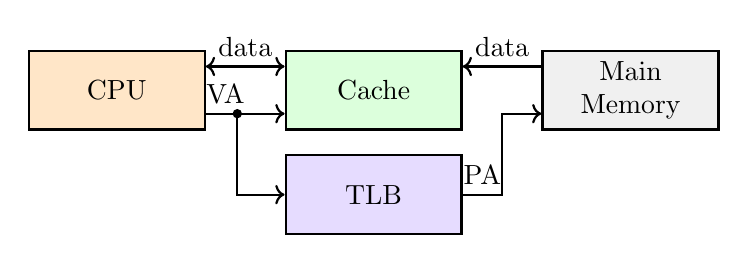
\begin{tikzpicture}[
    box/.style={rectangle, draw, thick, minimum width=1.8cm, minimum height=1cm, text centered, text width=2cm},
    data_connector/.style={circle, fill, inner sep=1.2pt},
    arrow/.style={->, thick, yshift=-2mm},
    doublearrow/.style={<->, thick, yshift=-2mm}]
    
    % Define colors
    \definecolor{cpucolor}{RGB}{255,230,200}
    \definecolor{cachecolor}{RGB}{220,255,220}
    \definecolor{tlbcolor}{RGB}{230,220,255}
    \definecolor{memcolor}{RGB}{240,240,240}
    
    % Nodes
    \node[box, fill=cpucolor] (cpu) {CPU};
    \node[box, fill=cachecolor, right=of cpu] (cache) {Cache};
    \node[box, fill=memcolor, align=center, right=of cache] (memory) {Main Memory};
    \node[box, fill=tlbcolor, below=3mm of cache] (tlb) {TLB};
    
    % Arrows with labels
    % CPU to Cache - bidirectional with VA going right, data going left
    %\draw[arrow] (cpu.east) -- node[above] {\small VA} (cache.west);
    %\draw[arrow] (cache.west) -- +(-0.7,0) -- +(-0.7,0.3) -- ($(cpu.east) + (0,0.3)$) -- node[above, pos=0.7] {\small data} (cpu.east |- {$(cpu.east) + (0,0.3)$});
    
    \draw[doublearrow] ([yshift=3mm]cache.west) -- node[above] {data} ([yshift=3mm]cpu.east);
    
    \draw[arrow] ([yshift=-3mm]cpu.east) -- node[above, near start] {VA} ([yshift=-3mm]cache.west);
    
    % TLB to Memory - PA
    \draw[arrow] (tlb.east) -- node[above] {PA} ++(0.5,0) |- ([yshift=-3mm]memory.west);
    \draw[arrow] ([yshift=3mm]memory.west) -- node[above] {data} ([yshift=3mm]cache.east);
    \draw[arrow] ([xshift=4mm, yshift=-3mm]cpu.east) node[data_connector] {} |- (tlb.west);
    
\end{tikzpicture}
\end{center}

\vspace{0.1cm}
\begin{itemize}
\item \textbf{Two virtual pages mapped to the same physical page}
    \begin{itemize}
    \item Must not reside in the cache together
    \item On a cache miss, use a reverse TLB to verify that no other cache line already in the cache mapped to the missed physical address
    \end{itemize}
    
\item \textbf{Flush cache on context switch}
    \begin{itemize}
    \item Alternatively: add process ID as part of the tag
    \end{itemize}
\end{itemize}
\end{frame}

\section{x86 Paging Implementation}

\begin{frame}{}
\begin{center}
\Huge Paging in x86
\end{center}
\end{frame}

\begin{frame}{Page Table Size -- The Problem}
\textbf{Assume a flat (single-level) page table:}
\begin{itemize}
\item Virtual address space: $2^{48}$ bytes
\item Page size: 4KB = $2^{12}$B $\rightarrow$ Number of pages: $\frac{2^{48}}{2^{12}} = 2^{36}$ entries
\item PTE size: 8 bytes $\rightarrow$ Page table size: $2^{36} \times 8$B = $2^{39}$B = \textbf{512GB per process!}
\item 128 processes $\rightarrow$ $2^{39} \times 128 = 2^{46}$B = \textbf{64TB just for page tables}
\end{itemize}
\vspace{3mm}
\textbf{Problem:} Page tables alone would require more memory than physically available
\end{frame}

\begin{frame}{Page Table Size -- Hierarchical Page Tables}
\textbf{Observation:} Most processes use only a small portion of the virtual address space
\vspace{2mm}

\textbf{Solution: Hierarchical Page Tables (Radix Tree)}
\begin{itemize}
\item Split the page table into a tree structure (multi-level)
\item Each level is indexed by a portion of the virtual address
\item Only allocate page table pages for address ranges actually in use
\item Sparse address spaces $\rightarrow$ sparse page tables
\end{itemize}
\vspace{2mm}

\textbf{Additional benefit:}
\begin{itemize}
\item Page table pages can themselves be paged out to disk
\item If accessing a missing page table page $\rightarrow$ CPU traps to OS to fetch it
\end{itemize}
\vspace{2mm}

\textbf{Other solutions exist:} Hashed page tables, inverted page tables, software-managed TLB
\end{frame}


\begin{frame}{4KB Page Mapping in 64-bit Mode}
\begin{columns}[T]
\begin{column}{0.44\textwidth}
\begin{itemize}
\item \textbf{4-level hierarchical paging}
\item Each page table: 4KB in size
\item Each page table entry (PTE): 8B
\item Entries per table: $\frac{4\text{KB}}{8\text{B}} = 512 = 2^9$
\item Level $n$ entry points to level $n-1$ table base
    \begin{itemize}
    \item[$\triangleright$] Provides $(M-12)$ address bits
    \item[$\triangleright$] Bits [11:0] = 0 (4KB-aligned)
    \item[$\triangleright$] $M = \log_2(\text{physical mem size})$
    \item[$\triangleright$] CR3 register $\rightarrow$ PML4 base
    \end{itemize}
\item 9 VA bits $\rightarrow$ index in each table
\item VA[11:0] byte offset in 4KB page
\end{itemize}
\end{column}

\begin{column}{0.56\textwidth}
\begin{center}
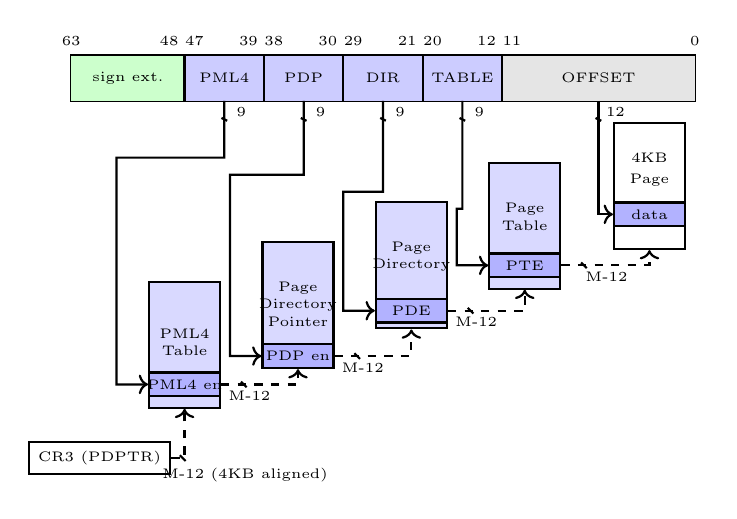
\begin{tikzpicture}[scale=0.72,
    table/.style={rectangle, draw, thick, minimum width=0.9cm, fill=blue!15},
    entry/.style={rectangle, draw, thick, minimum width=0.9cm, minimum height=0.3cm, fill=blue!30},
    data/.style={rectangle, draw, thick, minimum width=0.9cm, minimum height=1.6cm, fill=white},
    arrow/.style={->, thick},
    dashedarrow/.style={->, thick, dashed}]
    
    % Virtual Address breakdown at the top
    \draw[thick] (0,7.5) rectangle (11,8.3);
    
    % Address fields with colors
    \fill[green!20] (0,7.5) rectangle (2,8.3);
    \fill[blue!20] (2,7.5) rectangle (3.4,8.3);
    \fill[blue!20] (3.4,7.5) rectangle (4.8,8.3);
    \fill[blue!20] (4.8,7.5) rectangle (6.2,8.3);
    \fill[blue!20] (6.2,7.5) rectangle (7.6,8.3);
    \fill[gray!20] (7.6,7.5) rectangle (11,8.3);
    
    % Field separators
    \draw[thick] (2,7.5) -- (2,8.3);
    \draw[thick] (3.4,7.5) -- (3.4,8.3);
    \draw[thick] (4.8,7.5) -- (4.8,8.3);
    \draw[thick] (6.2,7.5) -- (6.2,8.3);
    \draw[thick] (7.6,7.5) -- (7.6,8.3);
    
    % Field labels above
    \node[above, font=\tiny] at (0,8.3) {63};
    \node[above, font=\tiny] at (1.95,8.3) {48 47};
    \node[above, font=\tiny] at (3.35,8.3) {39 38};
    \node[above, font=\tiny] at (4.75,8.3) {30 29};
    \node[above, font=\tiny] at (6.15,8.3) {21 20};
    \node[above, font=\tiny] at (7.55,8.3) {12 11};
    \node[above, font=\tiny] at (11,8.3) {0};
    
    \node[font=\tiny] at (1,7.9) {sign ext.};
    \node[font=\tiny] at (2.7,7.9) {PML4};
    \node[font=\tiny] at (4.1,7.9) {PDP};
    \node[font=\tiny] at (5.5,7.9) {DIR};
    \node[font=\tiny] at (6.9,7.9) {TABLE};
    \node[font=\tiny] at (9.3,7.9) {OFFSET};
    
    % Page table hierarchy - ascending from left to right with bigger vertical gaps
    % PML4 Table (lowest)
    \node[table, minimum height=1.6cm] (pml4) at (2,3.2) {};
    \node[font=\tiny] at (2,3.4) {PML4};
    \node[font=\tiny] at (2,3.1) {Table};
    \node[entry] (pml4en) at (2,2.5) {};
    \node[font=\tiny] at (pml4en) {PML4 en};
    
    % PDP Table (higher)
    \node[table, minimum height=1.6cm] (pdp) at (4,3.9) {};
    \node[font=\tiny] at (4,4.2) {Page};
    \node[font=\tiny] at (4,3.9) {Directory};
    \node[font=\tiny] at (4,3.6) {Pointer};
    \node[entry] (pdpen) at (4,3.0) {};
    \node[font=\tiny] at (pdpen) {PDP en};
    
    % Page Directory (higher)
    \node[table, minimum height=1.6cm] (dir) at (6,4.6) {};
    \node[font=\tiny] at (6,4.9) {Page};
    \node[font=\tiny] at (6,4.6) {Directory};
    \node[entry] (pde) at (6,3.8) {};
    \node[font=\tiny] at (pde) {PDE};
    
    % Page Table (even higher)
    \node[table, minimum height=1.6cm] (pt) at (8,5.3) {};
    \node[font=\tiny] at (8,5.6) {Page};
    \node[font=\tiny] at (8,5.3) {Table};
    \node[entry] (pte) at (8,4.6) {};
    \node[font=\tiny] at (pte) {PTE};
    
    % Data Page (highest) with data rectangle full width
    \node[data, minimum height=1.6cm] (datapage) at (10.2,6) {};
    \node[font=\tiny] at (10.2,6.5) {4KB};
    \node[font=\tiny] at (10.2,6.1) {Page};
    % Draw rectangle around "data" - full width of the page
    \node[entry] (databox) at (10.2,5.5) {};
    \node[font=\tiny] at (databox) {data};
    
    % CR3
    \node[rectangle, draw, thick, minimum width=1.2cm, minimum height=0.4cm] (cr3) at (0.5,1.2) {\tiny CR3 (PDPTR)};
    
    % Arrows from address fields to table entries (to west side) with "/" on line
    % PML4 arrow with "9" near origin and "/" on line
    \draw[arrow] (2.7,7.5) -- (2.7,6.5) -- (0.8,6.5) -- (0.8,2.5) -- (pml4en.west);
    \node[font=\tiny] at (3,7.3) {9};
    \draw[thick] (2.65,7.2) -- (2.75,7.15);
    
    % PDP arrow with "9" near origin and "/" on line
    \draw[arrow] (4.1,7.5) -- (4.1,6.2) -- (2.8,6.2) -- (2.8,3.0) -- (pdpen.west);
    \node[font=\tiny] at (4.4,7.3) {9};
    \draw[thick] (4.05,7.2) -- (4.15,7.15);
    
    % DIR arrow with "9" near origin and "/" on line
    \draw[arrow] (5.5,7.5) -- (5.5,5.9) -- (4.8,5.9) -- (4.8,3.8) -- (pde.west);
    \node[font=\tiny] at (5.8,7.3) {9};
    \draw[thick] (5.45,7.2) -- (5.55,7.15);
    
    % TABLE arrow with "9" near origin and "/" on line
    \draw[arrow] (6.9,7.5) -- (6.9,5.6) -- (6.8,5.6) -- (6.8,4.6) -- (pte.west);
    \node[font=\tiny] at (7.2,7.3) {9};
    \draw[thick] (6.85,7.2) -- (6.95,7.15);
    
    % OFFSET arrow to data box with "12" near origin and "/" on line
    \draw[arrow] (9.3,7.5) |- (databox.west);
    \node[font=\tiny] at (9.6,7.3) {12};
    \draw[thick] (9.25,7.2) -- (9.35,7.15);
    
    % Arrows connecting the hierarchy with bus width notation
    % CR3 to PML4 Table south (not PML4 en) - dashed
    \draw[dashedarrow] (cr3.east) -| (pml4.south);
    \draw[thick] ($(cr3.east) + (0.15,0.05)$) -- ($(cr3.east) + (0.25,-0.05)$);
    \node[font=\tiny] at ($(cr3.east) + (1.3,-0.3)$) {M-12 (4KB aligned)};
    
    % PML4 en to PDP Table south - dashed with "\" mark
    \draw[dashedarrow] (pml4en.east) -| (pdp.south);
    \draw[thick] ($(pml4en.east) + (0.35,0.05)$) -- ($(pml4en.east) + (0.45,-0.05)$);
    \node[font=\tiny] at ($(pml4en.east) + (0.5,-0.2)$) {M-12};
    
    % PDP en to Page Directory south - dashed with "\" mark
    \draw[dashedarrow] (pdpen.east) -| (dir.south);
    \draw[thick] ($(pdpen.east) + (0.35,0.05)$) -- ($(pdpen.east) + (0.45,-0.05)$);
    \node[font=\tiny] at ($(pdpen.east) + (0.5,-0.2)$) {M-12};
    
    % PDE to Page Table south - dashed with "\" mark
    \draw[dashedarrow] (pde.east) -| (pt.south);
    \draw[thick] ($(pde.east) + (0.35,0.05)$) -- ($(pde.east) + (0.45,-0.05)$);
    \node[font=\tiny] at ($(pde.east) + (0.5,-0.2)$) {M-12};
    
    % PTE to 4KByte Page (datapage) bottom - dashed with "\" mark
    \draw[dashedarrow] (pte.east) -| (datapage.south);
    \draw[thick] ($(pte.east) + (0.35,0.05)$) -- ($(pte.east) + (0.45,-0.05)$);
    \node[font=\tiny] at ($(pte.east) + (0.8,-0.2)$) {M-12};
    
\end{tikzpicture}
\end{center}
\end{column}
\end{columns}
\end{frame}


\begin{frame}{Example: Page Table Hierarchy}
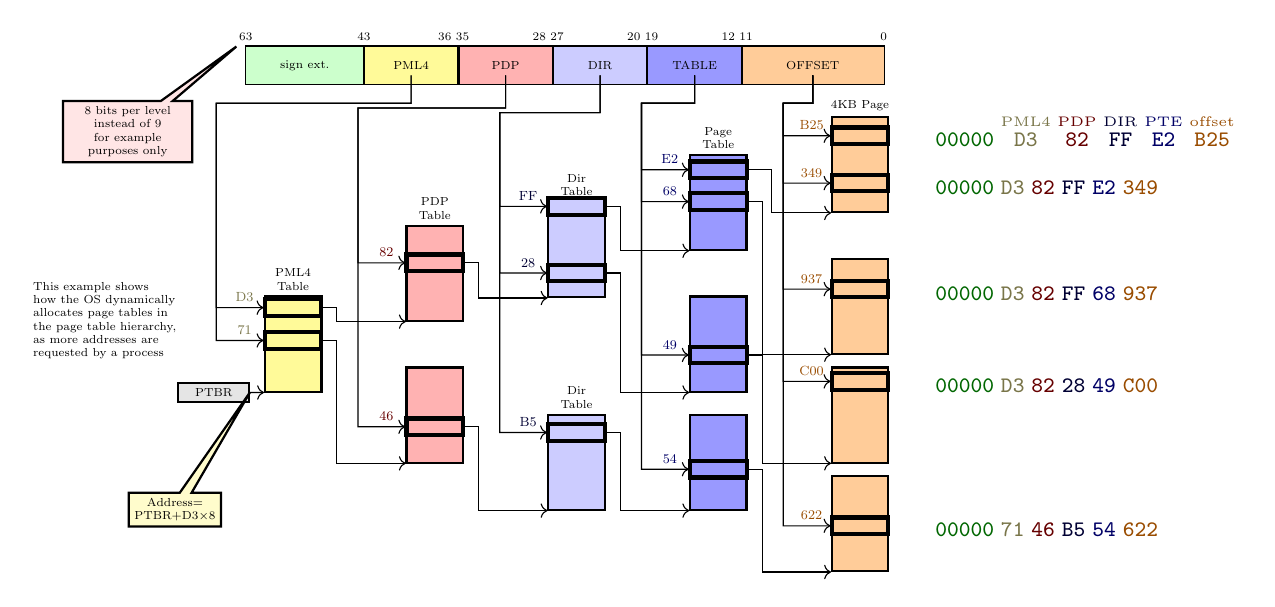
\begin{tikzpicture}[scale=0.6, transform shape,
    % Table styles for different levels
    pml4table/.style={rectangle, draw=black, thick, minimum width=1.2cm, minimum height=2.016cm, fill=yellow!40},
    pdptable/.style={rectangle, draw=black, thick, minimum width=1.2cm, minimum height=2.016cm, fill=red!30},
    dirtable/.style={rectangle, draw=black, thick, minimum width=1.2cm, minimum height=2.016cm, fill=blue!20},
    pagetable/.style={rectangle, draw=black, thick, minimum width=1.2cm, minimum height=2.016cm, fill=blue!40},
    page/.style={rectangle, draw=black, thick, minimum width=1.2cm, minimum height=2.016cm, fill=orange!40},
    % Entry styles for each level (smaller boxes with thick border)
    pml4entry/.style={rectangle, draw=black, line width=1.5pt, minimum width=1.2cm, minimum height=0.35cm, fill=yellow!40, anchor=south},
    pdpentry/.style={rectangle, draw=black, line width=1.5pt, minimum width=1.2cm, minimum height=0.35cm, fill=red!30, anchor=south},
    direntry/.style={rectangle, draw=black, line width=1.5pt, minimum width=1.2cm, minimum height=0.35cm, fill=blue!20, anchor=south},
    pageentry/.style={rectangle, draw=black, line width=1.5pt, minimum width=1.2cm, minimum height=0.35cm, fill=blue!40, anchor=south},
    pageoffset/.style={rectangle, draw=black, line width=1.5pt, minimum width=1.2cm, minimum height=0.35cm, fill=orange!40, anchor=south},
    arrow/.style={->, black},
    entrytag/.style={pos=0.6, above, font=\footnotesize},
    pml4tag/.style={pos=0.6, above, font=\footnotesize, text=yellow!40!black},
    pdptag/.style={pos=0.6, above, font=\footnotesize, text=red!40!black},
    dirtag/.style={pos=0.6, above, font=\footnotesize, text=blue!20!black},
    ptetag/.style={pos=0.6, above, font=\footnotesize, text=blue!40!black},
    offsettag/.style={pos=0.6, above, font=\footnotesize, text=orange!60!black}
]

% Top: Virtual Address breakdown
\draw[thick] (0,10.5) rectangle (13.5,11.3);

% Address field colors
\fill[green!20] (0,10.5) rectangle (2.5,11.3);
\fill[yellow!40] (2.5,10.5) rectangle (4.5,11.3);
\fill[red!30] (4.5,10.5) rectangle (6.5,11.3);
\fill[blue!20] (6.5,10.5) rectangle (8.5,11.3);
\fill[blue!40] (8.5,10.5) rectangle (10.5,11.3);
\fill[orange!40] (10.5,10.5) rectangle (13.5,11.3);

% Field separators
\draw[thick] (2.5,10.5) -- (2.5,11.3);
\draw[thick] (4.5,10.5) -- (4.5,11.3);
\draw[thick] (6.5,10.5) -- (6.5,11.3);
\draw[thick] (8.5,10.5) -- (8.5,11.3);
\draw[thick] (10.5,10.5) -- (10.5,11.3);

% Field labels above
\node[above, font=\scriptsize] at (0,11.3) {63};
\node[above, font=\scriptsize] at (2.5,11.3) {43};
\node[above, font=\scriptsize] at (4.4,11.3) {36 35};
\node[above, font=\scriptsize] at (6.4,11.3) {28 27};
\node[above, font=\scriptsize] at (8.4,11.3) {20 19};
\node[above, font=\scriptsize] at (10.4,11.3) {12 11};
\node[above, font=\scriptsize] at (13.5,11.3) {0};

% Field names inside
\node[font=\scriptsize] at (1.25,10.9) {sign ext.};
\node[font=\scriptsize] (pml4label) at (3.5,10.9) {PML4};
\node[font=\scriptsize] (pdplabel) at (5.5,10.9) {PDP};
\node[font=\scriptsize] (dirlabel) at (7.5,10.9) {DIR};
\node[font=\scriptsize] (tablelabel) at (9.5,10.9) {TABLE};
\node[font=\scriptsize] (offsetlabel) at (12,10.9) {OFFSET};

% Vertical alignment of tables (from left to right)
% PML4 Table
\node[pml4table] (pml4base) at (1,5) {};
\node[font=\scriptsize, anchor=south, align=center] at (pml4base.north) {PML4\\ Table};
\node[pml4entry] (pml4d3) at ($(pml4base.south)!0.78!(pml4base.north)$) {}; % D3 = 211/255, reduced by 15%
\node[pml4entry] (pml471) at ($(pml4base.south)!0.44!(pml4base.north)$) {}; % 71 = 113/255

% PTBR register pointing to PML4
\node[rectangle, draw=black, thick, fill=gray!20, minimum width=1.5cm, minimum height=0.4cm, font=\scriptsize, anchor=east] (cr3) at ([xshift=-3mm]pml4base.south west) {PTBR};
\draw[arrow] (cr3) -- (pml4base.south west);

% Address calculation label
\node[font=\scriptsize, draw=black, thick, fill=yellow!20, align=center,
      rectangle callout, callout absolute pointer={(cr3.east)}] at (-1.5,1.5) {Address=\\ PTBR+D3$\times$8};

% PDP Table (2 instances)
\node[pdptable] (pdp82base) at (4,6.5) {};
\node[font=\scriptsize, anchor=south, align=center] at (pdp82base.north) {PDP\\ Table};
\node[pdpentry] (pdp82) at ($(pdp82base.south)!0.51!(pdp82base.north)$) {}; % 82 = 130/255

\node[pdptable] (pdp46base) at (4,3.5) {};
\node[pdpentry] (pdp46) at ($(pdp46base.south)!0.28!(pdp46base.north)$) {}; % 46 = 70/255

% Page Dir instances
\node[dirtable] (dirffbase) at (7,7) {};
\node[font=\scriptsize, anchor=south, align=center] at (dirffbase.north) {Dir\\ Table};
\node[direntry] (dirff) at ($(dirffbase.south)!0.85!(dirffbase.north)$) {}; % FF = 255/255, reduced by 15%
\node[direntry] (dir28) at ($(dirffbase.south)!0.16!(dirffbase.north)$) {}; % 28 = 40/255

\node[dirtable] (dirb5base) at (7,2.5) {};
\node[font=\scriptsize, anchor=south, align=center] at (dirb5base.north) {Dir\\ Table};
\node[direntry] (dirb5) at ($(dirb5base.south)!0.71!(dirb5base.north)$) {}; % B5 = 181/255

% Page Table instances
\node[pagetable] (pte2base) at (10,8) {};
\node[font=\scriptsize, anchor=south, align=center] at (pte2base.north) {Page\\ Table};
\node[pageentry] (ptee2) at ($(pte2base.south)!0.74!(pte2base.north)$) {}; % E2 = 226/255, reduced by 15%
\node[pageentry] (pte68) at ($(pte2base.south)!0.41!(pte2base.north)$) {}; % 68 = 104/255

\node[pagetable] (pte49base) at (10,5) {};
\node[pageentry] (pte49) at ($(pte49base.south)!0.29!(pte49base.north)$) {}; % 49 = 73/255

\node[pagetable] (pte54base) at (10,2.5) {};
\node[pageentry] (pte54) at ($(pte54base.south)!0.33!(pte54base.north)$) {}; % 54 = 84/255

% 4KB Pages with offsets
\node[page] (pageb25base) at (13,8.8) {};
\node[font=\scriptsize, anchor=south] at (pageb25base.north) {4KB Page};
\node[pageoffset] (pageb25) at ($(pageb25base.south)!0.70!(pageb25base.north)$) {}; % B25 = 2853/4095
\node[pageoffset] (page349) at ($(pageb25base.south)!0.21!(pageb25base.north)$) {}; % 349 = 841/4095

\node[page] (page937base) at (13,5.8) {};
\node[pageoffset] (page937) at ($(page937base.south)!0.58!(page937base.north)$) {}; % 937 = 2359/4095

\node[page] (pagec00base) at (13,3.5) {};
\node[pageoffset] (pagec00) at ($(pagec00base.south)!0.75!(pagec00base.north)$) {}; % C00 = 3072/4095

\node[page] (page622base) at (13,1.2) {};
\node[pageoffset] (page622) at ($(page622base.south)!0.38!(page622base.north)$) {}; % 622 = 1570/4095

% Paths from address fields to table entries
% PML4 entries
\draw[arrow] (pml4label) -- ++(0, -0.8) -| ([xshift=-10mm]pml4d3.west) -- (pml4d3.west) node[pml4tag] {D3};
\draw[arrow] (pml4label) -- ++(0, -0.8) -| ([xshift=-10mm]pml471.west) -- (pml471.west) node[pml4tag] {71};

% PDP entries
\draw[arrow] (pdplabel) -- ++(0, -0.9) -| ([xshift=-10mm]pdp82.west) -- (pdp82.west) node[pdptag] {82};
\draw[arrow] (pdplabel) -- ++(0, -0.9) -| ([xshift=-10mm]pdp46.west) -- (pdp46.west) node[pdptag] {46};

% DIR entries
\draw[arrow] (dirlabel) -- ++(0, -1) -| ([xshift=-10mm]dirff.west) -- (dirff.west) node[dirtag] {FF};
\draw[arrow] (dirlabel) -- ++(0, -1) -| ([xshift=-10mm]dir28.west) -- (dir28.west) node[dirtag] {28};
\draw[arrow] (dirlabel) -- ++(0, -1) -| ([xshift=-10mm]dirb5.west) -- (dirb5.west) node[dirtag] {B5};

% TABLE entries
\draw[arrow] (tablelabel) -- ++(0, -0.8) -| ([xshift=-10mm]ptee2.west) -- (ptee2.west) node[ptetag] {E2};
\draw[arrow] (tablelabel) -- ++(0, -0.8) -| ([xshift=-10mm]pte68.west) -- (pte68.west) node[ptetag] {68};
\draw[arrow] (tablelabel) -- ++(0, -0.8) -| ([xshift=-10mm]pte49.west) -- (pte49.west) node[ptetag] {49};
\draw[arrow] (tablelabel) -- ++(0, -0.8) -| ([xshift=-10mm]pte54.west) -- (pte54.west) node[ptetag] {54};

% OFFSET entries
\draw[arrow] (offsetlabel) -- ++(0, -0.8) -| ([xshift=-10mm]pageb25.west) -- (pageb25.west) node[offsettag] {B25};
\draw[arrow] (offsetlabel) -- ++(0, -0.8) -| ([xshift=-10mm]page349.west) -- (page349.west) node[offsettag] {349};
\draw[arrow] (offsetlabel) -- ++(0, -0.8) -| ([xshift=-10mm]page937.west) -- (page937.west) node[offsettag] {937};
\draw[arrow] (offsetlabel) -- ++(0, -0.8) -| ([xshift=-10mm]pagec00.west) -- (pagec00.west) node[offsettag] {C00};
\draw[arrow] (offsetlabel) -- ++(0, -0.8) -| ([xshift=-10mm]page622.west) -- (page622.west) node[offsettag] {622};

% Arrows connecting the hierarchy
% PML4[D3] -> PDP[82]
\draw[arrow] (pml4d3.east) -- ++(0.3, 0) |- (pdp82base.south west);
% PML4[71] -> PDP[46]
\draw[arrow] (pml471.east) -- ++(0.3, 0) |- (pdp46base.south west);

% PDP[82] -> Dir[FF,28]
\draw[arrow] (pdp82.east) -- ++(0.3, 0) |- (dirffbase.south west);
% PDP[46] -> Dir[B5]
\draw[arrow] (pdp46.east) -- ++(0.3, 0) |- (dirb5base.south west);

% Dir[FF] -> PT[E2,68]
\draw[arrow] (dirff.east) -- ++(0.3, 0) |- (pte2base.south west);
% Dir[28] -> PT[49]
\draw[arrow] (dir28.east) -- ++(0.3, 0) |- (pte49base.south west);
% Dir[B5] -> PT[54]
\draw[arrow] (dirb5.east) -- ++(0.3, 0) |- (pte54base.south west);

% PT[E2] -> Page[B25,349]
\draw[arrow] (ptee2.east) -- ++(0.5, 0) |- (pageb25base.south west);
% PT[68] -> Page[937]
\draw[arrow] (pte68.east) -- ++(0.3, 0) |- (page937base.south west);
% PT[49] -> Page[C00]
\draw[arrow] (pte49.east) -- ++(0.3, 0) |- (pagec00base.south west);
% PT[54] -> Page[622]
\draw[arrow] (pte54.east) -- ++(0.3, 0) |- (page622base.south west);

% Right side: Complete virtual addresses (color-coded) - positioned relative to page entries
% First address with labels (2-row matrix)
\matrix[anchor=south west, matrix of nodes, nodes={draw=none, inner sep=1pt, font=\footnotesize\ttfamily},
        column sep=0.5pt, row sep=0.5pt, ampersand replacement=\&] (addr1) at ([xshift=7mm,yshift=-3mm]pageb25.south east) {
    |[font=\fontsize{4pt}{5pt}\selectfont]| {} \&
    |[font=\fontsize{4pt}{5pt}\selectfont, text=yellow!40!black]| PML4 \&
    |[font=\fontsize{4pt}{5pt}\selectfont, text=red!40!black]| PDP \&
    |[font=\fontsize{4pt}{5pt}\selectfont, text=blue!20!black]| DIR \&
    |[font=\fontsize{4pt}{5pt}\selectfont, text=blue!40!black]| PTE \&
    |[font=\fontsize{4pt}{5pt}\selectfont, text=orange!60!black]| offset \\
    |[text=green!40!black]| 00000 \&
    |[text=yellow!40!black]| D3 \&
    |[text=red!40!black]| 82 \&
    |[text=blue!20!black]| FF \&
    |[text=blue!40!black]| E2 \&
    |[text=orange!60!black]| B25 \\
};

% Other addresses (single-row matrices)
\matrix[anchor=south west, matrix of nodes, nodes={draw=none, inner sep=1pt, font=\footnotesize\ttfamily},
        column sep=0.5pt, ampersand replacement=\&] at ([xshift=7mm,yshift=-3mm]page349.south east) {
    |[text=green!40!black]| 00000 \&
    |[text=yellow!40!black]| D3 \&
    |[text=red!40!black]| 82 \&
    |[text=blue!20!black]| FF \&
    |[text=blue!40!black]| E2 \&
    |[text=orange!60!black]| 349 \\
};

\matrix[anchor=south west, matrix of nodes, nodes={draw=none, inner sep=1pt, font=\footnotesize\ttfamily},
        column sep=0.5pt, ampersand replacement=\&] at ([xshift=7mm,yshift=-3mm]page937.south east) {
    |[text=green!40!black]| 00000 \&
    |[text=yellow!40!black]| D3 \&
    |[text=red!40!black]| 82 \&
    |[text=blue!20!black]| FF \&
    |[text=blue!40!black]| 68 \&
    |[text=orange!60!black]| 937 \\
};

\matrix[anchor=south west, matrix of nodes, nodes={draw=none, inner sep=1pt, font=\footnotesize\ttfamily},
        column sep=0.5pt, ampersand replacement=\&] at ([xshift=7mm,yshift=-3mm]pagec00.south east) {
    |[text=green!40!black]| 00000 \&
    |[text=yellow!40!black]| D3 \&
    |[text=red!40!black]| 82 \&
    |[text=blue!20!black]| 28 \&
    |[text=blue!40!black]| 49 \&
    |[text=orange!60!black]| C00 \\
};

\matrix[anchor=south west, matrix of nodes, nodes={draw=none, inner sep=1pt, font=\footnotesize\ttfamily},
        column sep=0.5pt, ampersand replacement=\&] at ([xshift=7mm,yshift=-3mm]page622.south east) {
    |[text=green!40!black]| 00000 \&
    |[text=yellow!40!black]| 71 \&
    |[text=red!40!black]| 46 \&
    |[text=blue!20!black]| B5 \&
    |[text=blue!40!black]| 54 \&
    |[text=orange!60!black]| 622 \\
};

% Note about 8 bits
\node[font=\scriptsize, draw=black, thick, fill=red!10, align=center, text width=2.5cm,
      rectangle callout, callout absolute pointer={(-0.2,11.3)}] at (-2.5,9.5) {8 bits per level instead of 9 for example purposes only};

% Bottom left: Note about OS dynamic allocation
\node[font=\scriptsize, text width=4cm, align=left] at (-2.5,5.5) {
This example shows\\
how the OS dynamically\\
allocates page tables in\\
the page table hierarchy,\\
as more addresses are\\
requested by a process
};

\end{tikzpicture}
\end{frame}

\section{Advanced TLB Topics}

\begin{frame}{TLBs}
\textbf{The most recently used PDEs and PTEs are cached in TLBs}
\begin{itemize}
\item Separate TLB for data and instruction caches
\item Separate TLBs for 4KB, 2/4MB and 1GB page sizes
\item 2nd level TLB serves both instruction TLB and data TLB
\item TLB sizes in 6th Generation Intel® Core™ Processors:
\end{itemize}

\begin{center}
\footnotesize
\begin{tabular}{|l|c|c|c|}
\hline
 & \textbf{4KB pages} & \textbf{2MB/4MB Pages} & \textbf{1GB Pages} \\
\hline
Instruction TLBs & 128 entries, 8 ways & 8 entries / thread & none \\
\hline
Data TLBs & 64 entries, 4 ways & 32 entries, 4 ways & 4 entries, 4 ways \\
\hline
2nd level TLB & \multicolumn{2}{c|}{1536 entries, 12 ways (Shared by 4KB and 2/4MB pages)} & 16 entries, 4 ways \\
\hline
\end{tabular}
\end{center}

\textbf{In case of a hit in multiple TLBs}
\begin{itemize}
\item The largest page that hits is used
\end{itemize}
\end{frame}

\begin{frame}{PMH – Page Miss Handler}
\textbf{In case of an iTLB or a dTLB miss $\rightarrow$ Request PTE from PMH}
\begin{itemize}
\item PMH first tries the STLB (2nd level TLB) – save walk in case of an STLB hit
\item If STLB miss, PMH performs a page-walk: traverses the page table tree, starting at the root
\end{itemize}

\textbf{The PMH includes caches to shorten the page walk time}
\begin{itemize}
\item All 3 caches are accessed in parallel – use hit from the lowest table that hits
\item For each table that needs memory access PMH injects a "load"
\end{itemize}

\begin{center}
\footnotesize
\begin{tabular}{|l|l|l|l|}
\hline
\thead{cache} & \thead{Accessed with \\ VA bits} & \thead{If hits, \\ returns} & \thead{Saves accesses \\ to tables} \\
\hline
PDE cache & [47:21] & PDE & PTE \\
\hline
PDP cache & [47:30] & PDP entry & PDE and PTE \\
\hline
PML4 cache & [47:39] & PML4 entry & PDP, PDE, and PTE \\
\hline
\end{tabular}
\end{center}

\textbf{Page attributes}
\begin{itemize}
\item R/W flag: logical AND of R/W flag in all levels
\item U/S flag: logical OR of U/S flag in all levels
\item XD flag: logical OR of XD flag in all levels
\end{itemize}
\end{frame}

\begin{frame}{PMH: Page Walk Flowchart}
\centering
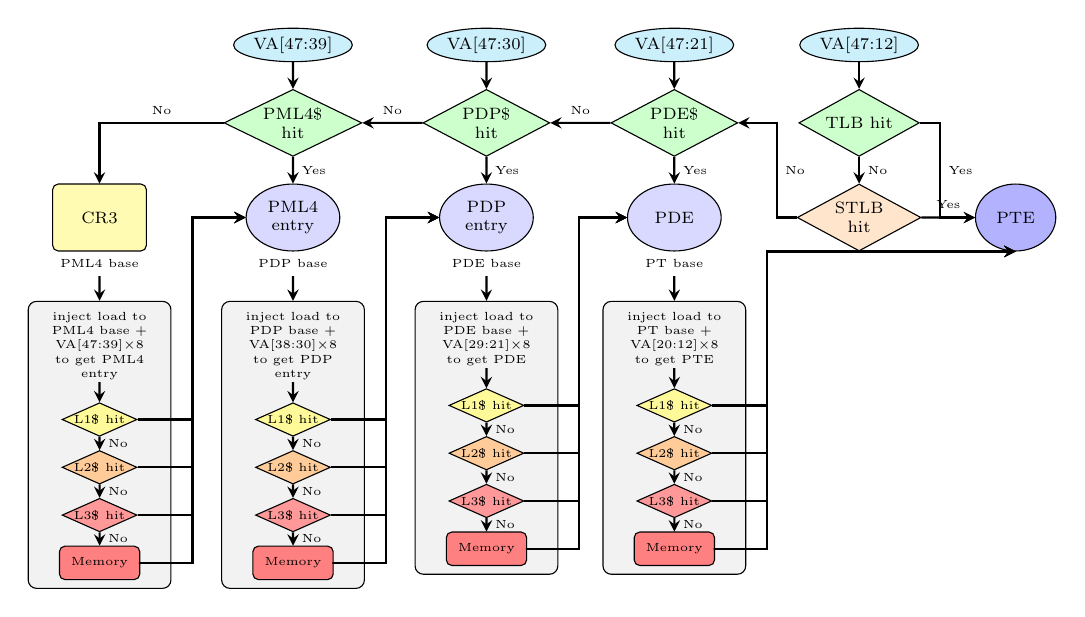
\begin{tikzpicture}[
    scale=0.85, transform shape,
    node distance=2mm,
    vabox/.style={ellipse, draw, fill=cyan!20, font=\scriptsize, inner sep=1pt, minimum width=14mm, minimum height=5mm},
    cachehit/.style={diamond, draw, fill=green!20, font=\scriptsize, inner sep=0pt, aspect=2.5, align=center, minimum width=18mm, minimum height=10mm},
    stlbhit/.style={diamond, draw, fill=orange!20, font=\scriptsize, inner sep=0pt, aspect=2.5, align=center, minimum width=18mm, minimum height=10mm},
    entrybox/.style={ellipse, draw, fill=blue!15, font=\scriptsize, inner sep=1pt, align=center, minimum width=14mm, minimum height=10mm},
    loadtext/.style={font=\tiny, text width=1.8cm, align=center, inner sep=1pt},
    basebox/.style={rectangle, draw, fill=yellow!30, font=\scriptsize, inner sep=2pt, rounded corners=2pt, minimum width=14mm, minimum height=10mm},
    l1hit/.style={diamond, draw, fill=yellow!40, font=\tiny, inner sep=0pt, aspect=2.5, minimum width=10mm, minimum height=5mm},
    l2hit/.style={diamond, draw, fill=orange!40, font=\tiny, inner sep=0pt, aspect=2.5, minimum width=10mm, minimum height=5mm},
    l3hit/.style={diamond, draw, fill=red!40, font=\tiny, inner sep=0pt, aspect=2.5, minimum width=10mm, minimum height=5mm},
    membox/.style={rectangle, draw, fill=red!50, font=\tiny, inner sep=2pt, rounded corners=2pt, minimum width=12mm, minimum height=5mm},
    ptebox/.style={ellipse, draw, fill=blue!30, font=\scriptsize, inner sep=2pt, minimum width=12mm, minimum height=10mm},
    fitbox/.style={draw, rounded corners=3pt, fill=gray!10, inner sep=3pt},
    arrow/.style={->, >=stealth, thick},
    ymark/.style={font=\tiny},
    nmark/.style={font=\tiny},
]

% Column 4: TLB (rightmost, placed first as reference)
\node[vabox] (va4) {VA[47:12]};
\node[cachehit, below=4mm of va4] (tlbhit) {TLB hit};
\node[stlbhit, below=4mm of tlbhit] (stlbhit) {STLB\\hit};

% PTE output (to the right of STLB)
\node[ptebox, right=8mm of stlbhit] (pte) {PTE};

% Column 3: PDE (left of TLB)
\node[cachehit, left=9mm of tlbhit] (pdehit) {PDE\$\\hit};
\node[vabox, above=4mm of pdehit] (va3) {VA[47:21]};
\node[entrybox, below=4mm of pdehit] (pdee) {PDE};
\node[font=\tiny, below=0pt of pdee] (pdeelabel) {PT base};
% PT inject/cache chain (below PDE)
\node[loadtext, below=5mm of pdeelabel] (ptload) {inject load to\\PT base +\\VA[20:12]$\times$8\\to get PTE};
\node[l1hit, below=3mm of ptload] (ptl1) {L1\$ hit};
\node[l2hit, below=2mm of ptl1] (ptl2) {L2\$ hit};
\node[l3hit, below=2mm of ptl2] (ptl3) {L3\$ hit};
\node[membox, below=2mm of ptl3] (ptmem) {Memory};

% Column 2: PDP (left of PDE)
\node[cachehit, left=9mm of pdehit] (pdphit) {PDP\$\\hit};
\node[vabox, above=4mm of pdphit] (va2) {VA[47:30]};
\node[entrybox, below=4mm of pdphit] (pdpe) {PDP\\entry};
\node[font=\tiny, below=0pt of pdpe] (pdpelabel) {PDE base};
% PDE inject/cache chain (below PDP entry)
\node[loadtext, below=5mm of pdpelabel] (pdeload) {inject load to\\PDE base +\\VA[29:21]$\times$8\\to get PDE};
\node[l1hit, below=3mm of pdeload] (pdel1) {L1\$ hit};
\node[l2hit, below=2mm of pdel1] (pdel2) {L2\$ hit};
\node[l3hit, below=2mm of pdel2] (pdel3) {L3\$ hit};
\node[membox, below=2mm of pdel3] (pdemem) {Memory};

% Column 1: PML4 (left of PDP)
\node[cachehit, left=9mm of pdphit] (pml4hit) {PML4\$\\hit};
\node[vabox, above=4mm of pml4hit] (va1) {VA[47:39]};
\node[entrybox, below=4mm of pml4hit] (pml4e) {PML4\\entry};
\node[font=\tiny, below=0pt of pml4e] (pml4elabel) {PDP base};
% PDP inject/cache chain (below PML4 entry)
\node[loadtext, below=5mm of pml4elabel] (pdpload) {inject load to\\PDP base +\\VA[38:30]$\times$8\\to get PDP\\entry};
\node[l1hit, below=3mm of pdpload] (pdpl1) {L1\$ hit};
\node[l2hit, below=2mm of pdpl1] (pdpl2) {L2\$ hit};
\node[l3hit, below=2mm of pdpl2] (pdpl3) {L3\$ hit};
\node[membox, below=2mm of pdpl3] (pdpmem) {Memory};

% Column 0: CR3 (same distance from pml4e as pdpe is from pml4e)
\node[basebox] at ($(pml4e)!-1!(pdpe)$) (cr3) {CR3};
\node[font=\tiny, below=0pt of cr3] (cr3label) {PML4 base};
% PML4 inject/cache chain (below CR3)
\node[loadtext, below=5mm of cr3label] (pml4load) {inject load to\\PML4 base +\\VA[47:39]$\times$8\\to get PML4\\entry};
\node[l1hit, below=3mm of pml4load] (pml4l1) {L1\$ hit};
\node[l2hit, below=2mm of pml4l1] (pml4l2) {L2\$ hit};
\node[l3hit, below=2mm of pml4l2] (pml4l3) {L3\$ hit};
\node[membox, below=2mm of pml4l3] (pml4mem) {Memory};

% Fit boxes around load text and cache chain
\begin{scope}[on background layer]
\node[fitbox, fit=(pml4load)(pml4l1)(pml4l2)(pml4l3)(pml4mem)] (pml4fit) {};
\node[fitbox, fit=(pdpload)(pdpl1)(pdpl2)(pdpl3)(pdpmem)] (pdpfit) {};
\node[fitbox, fit=(pdeload)(pdel1)(pdel2)(pdel3)(pdemem)] (pdefit) {};
\node[fitbox, fit=(ptload)(ptl1)(ptl2)(ptl3)(ptmem)] (ptfit) {};
\end{scope}

% Midpoint coordinates for cache chain arrows
\coordinate (pml4mid) at ($(pml4l1.east)!0.5!(pml4mem.east)$);
\coordinate (pdpmid) at ($(pdpl1.east)!0.5!(pdpmem.east)$);
\coordinate (pdemid) at ($(pdel1.east)!0.5!(pdemem.east)$);
\coordinate (ptmid) at ($(ptl1.east)!0.5!(ptmem.east)$);

% Arrows from VA to cache/TLB diamonds
\draw[arrow] (va1) -- (pml4hit);
\draw[arrow] (va2) -- (pdphit);
\draw[arrow] (va3) -- (pdehit);
\draw[arrow] (va4) -- (tlbhit);

% Yes arrows (cache hits go to entry)
\draw[arrow] (pml4hit) -- node[right, ymark] {Yes} (pml4e);
\draw[arrow] (pdphit) -- node[right, ymark] {Yes} (pdpe);
\draw[arrow] (pdehit) -- node[right, ymark] {Yes} (pdee);

% TLB/STLB Yes arrows to PTE
\draw[arrow] (tlbhit) -- node[right, nmark] {No} (stlbhit);
\draw[arrow] (tlbhit.east) -- ++(0.3,0) |- node[near start, right, ymark] {Yes} (pte);
\draw[arrow] (stlbhit.east) -- node[above, ymark] {Yes} (pte);

% No arrows (go left to previous level)
\draw[arrow] (pml4hit.west) -| node[near start, above, nmark] {No} (cr3.north);
\draw[arrow] (pdphit.west) -- node[above, nmark] {No} (pml4hit.east);
\draw[arrow] (pdehit.west) -- node[above, nmark] {No} (pdphit.east);
\draw[arrow] (stlbhit.west) -- ++(-0.3,0) |- node[near start, right, nmark] {No} (pdehit.east);

% CR3 to fit box
\draw[arrow] (cr3label.south) -- (pml4fit.north);

% Entry to fit box arrows (from base labels)
\draw[arrow] (pml4elabel.south) -- (pdpfit.north);
\draw[arrow] (pdpelabel.south) -- (pdefit.north);
\draw[arrow] (pdeelabel.south) -- (ptfit.north);

% Cache chain arrows (inside fit boxes)
\draw[arrow] (pml4load) -- (pml4l1);
\draw[arrow] (pml4l1) -- node[right, nmark] {No} (pml4l2);
\draw[arrow] (pml4l2) -- node[right, nmark] {No} (pml4l3);
\draw[arrow] (pml4l3) -- node[right, nmark] {No} (pml4mem);

\draw[arrow] (pdpload) -- (pdpl1);
\draw[arrow] (pdpl1) -- node[right, nmark] {No} (pdpl2);
\draw[arrow] (pdpl2) -- node[right, nmark] {No} (pdpl3);
\draw[arrow] (pdpl3) -- node[right, nmark] {No} (pdpmem);

\draw[arrow] (pdeload) -- (pdel1);
\draw[arrow] (pdel1) -- node[right, nmark] {No} (pdel2);
\draw[arrow] (pdel2) -- node[right, nmark] {No} (pdel3);
\draw[arrow] (pdel3) -- node[right, nmark] {No} (pdemem);

\draw[arrow] (ptload) -- (ptl1);
\draw[arrow] (ptl1) -- node[right, nmark] {No} (ptl2);
\draw[arrow] (ptl2) -- node[right, nmark] {No} (ptl3);
\draw[arrow] (ptl3) -- node[right, nmark] {No} (ptmem);

% Cache hits go to next entry (via midpoint, +3mm right before turning up)
\draw[arrow] (pml4l1.east) -- (pml4l1.east -| pml4mid) -- ++(0.8,0) |- (pml4e.west);
\draw[arrow] (pml4l2.east) -- (pml4l2.east -| pml4mid) -- ++(0.8,0) |- (pml4e.west);
\draw[arrow] (pml4l3.east) -- (pml4l3.east -| pml4mid) -- ++(0.8,0) |- (pml4e.west);
\draw[arrow] (pml4mem.east) -- (pml4mem.east -| pml4mid) -- ++(0.8,0) |- (pml4e.west);

\draw[arrow] (pdpl1.east) -- (pdpl1.east -| pdpmid) -- ++(0.8,0) |- (pdpe.west);
\draw[arrow] (pdpl2.east) -- (pdpl2.east -| pdpmid) -- ++(0.8,0) |- (pdpe.west);
\draw[arrow] (pdpl3.east) -- (pdpl3.east -| pdpmid) -- ++(0.8,0) |- (pdpe.west);
\draw[arrow] (pdpmem.east) -- (pdpmem.east -| pdpmid) -- ++(0.8,0) |- (pdpe.west);

\draw[arrow] (pdel1.east) -- (pdel1.east -| pdemid) -- ++(0.8,0) |- (pdee.west);
\draw[arrow] (pdel2.east) -- (pdel2.east -| pdemid) -- ++(0.8,0) |- (pdee.west);
\draw[arrow] (pdel3.east) -- (pdel3.east -| pdemid) -- ++(0.8,0) |- (pdee.west);
\draw[arrow] (pdemem.east) -- (pdemem.east -| pdemid) -- ++(0.8,0) |- (pdee.west);

% PT cache chain goes to PTE (via midpoint, +3mm right before turning up)
\draw[arrow] (ptl1.east) -- (ptl1.east -| ptmid) -- ++(0.8,0) |- (pte.south);
\draw[arrow] (ptl2.east) -- (ptl2.east -| ptmid) -- ++(0.8,0) |- (pte.south);
\draw[arrow] (ptl3.east) -- (ptl3.east -| ptmid) -- ++(0.8,0) |- (pte.south);
\draw[arrow] (ptmem.east) -- (ptmem.east -| ptmid) -- ++(0.8,0) |- (pte.south);

\end{tikzpicture}
\end{frame}

\begin{frame}{Translation Page Not Present}
\textbf{During a page walk, a translation hierarchy may return an entry with Present = 0}
\begin{itemize}
\item The page of translations pointed by this entry is not present in memory
\item PMH gets a page fault $\rightarrow$ the original load (not the PMH-injected load) faults to the OS
\item OS gets the missing translation page into memory
\item The load is re-fetched (and the PMH performs the walk again)
    \begin{itemize}
    \item The OS uses unused bits in the entry to encode the page location in the disk
    \item Most likely the lower pages in the hierarchy are also not be present
    \item OS brings all missing pages as part handling the same page fault
    \end{itemize}
\end{itemize}

\textbf{CR3 does not have a "present" bit}
\begin{itemize}
\item The PML4 table, which uses a single 4K page, is always present
\end{itemize}
\end{frame}

\begin{frame}{Cache and Translation Structures}
\begin{center}
[Diagram showing Core with PMH, L1 I\$ 32KB 8 ways, L1 D\$ 32KB 8 ways, MLC 256KB 4 ways, LLC 2MB per core, DRAM 8GB, and various TLB structures]
\end{center}
\end{frame}

% Additional advanced topics
% TEMPORARILY COMMENTED OUT - Global TLB Entries frame with matrix issues
\begin{comment}
\begin{frame}{Global TLB Entries}
\begin{columns}[T]
\begin{column}{0.48\textwidth}
\textbf{Problem:} Some pages used by all processes
\begin{itemize}
\item Kernel code pages
\item Shared libraries (libc, etc.)
\item System call handlers
\item Interrupt handlers
\end{itemize}

\textbf{Solution: Global bit in TLB}
\begin{itemize}
\item G bit in page table entry
\item TLB entry marked as global
\item Not flushed on context switch
\item Remains valid across all ASIDs
\end{itemize}
\end{column}

\begin{column}{0.52\textwidth}
\textbf{TLB Entry with Global Bit:}
\begin{center}
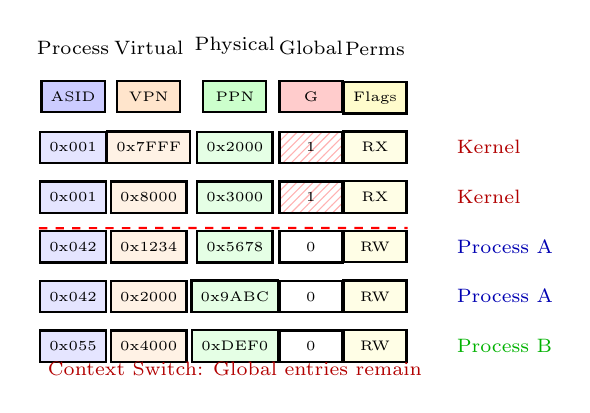
\begin{tikzpicture}[scale=0.9]
    % Define styles
    \tikzset{
        entry/.style={draw, thick, minimum height=0.4cm},
        globalentry/.style={entry, pattern=north east lines, pattern color=red!30}
    }
    
    % TLB structure as matrix
    \matrix[matrix of nodes, nodes={entry, minimum width=0.8cm}, 
            column sep=-\pgflinewidth, row sep=2mm,
            font=\tiny, ampersand replacement=\&] (tlb) {
        |[fill=blue!20]| ASID \& |[fill=orange!20]| VPN \& |[fill=green!20]| PPN \& |[fill=red!20]| G \& |[fill=yellow!20]| Flags \\
        |[fill=blue!10]| 0x001 \& |[fill=orange!10]| 0x7FFF \& |[fill=green!10]| 0x2000 \& |[globalentry]| 1 \& |[fill=yellow!10]| RX \\
        |[fill=blue!10]| 0x001 \& |[fill=orange!10]| 0x8000 \& |[fill=green!10]| 0x3000 \& |[globalentry]| 1 \& |[fill=yellow!10]| RX \\
        |[fill=blue!10]| 0x042 \& |[fill=orange!10]| 0x1234 \& |[fill=green!10]| 0x5678 \& 0 \& |[fill=yellow!10]| RW \\
        |[fill=blue!10]| 0x042 \& |[fill=orange!10]| 0x2000 \& |[fill=green!10]| 0x9ABC \& 0 \& |[fill=yellow!10]| RW \\
        |[fill=blue!10]| 0x055 \& |[fill=orange!10]| 0x4000 \& |[fill=green!10]| 0xDEF0 \& 0 \& |[fill=yellow!10]| RW \\
    };
    
    % Labels
    \node[above=2mm of tlb-1-1] {\scriptsize Process};
    \node[above=2mm of tlb-1-2] {\scriptsize Virtual};
    \node[above=2mm of tlb-1-3] {\scriptsize Physical};
    \node[above=2mm of tlb-1-4] {\scriptsize Global};
    \node[above=2mm of tlb-1-5] {\scriptsize Perms};
    
    % Annotations
    \node[right=5mm of tlb-2-5, text=red!70!black] {\scriptsize Kernel};
    \node[right=5mm of tlb-3-5, text=red!70!black] {\scriptsize Kernel};
    \node[right=5mm of tlb-4-5, text=blue!70!black] {\scriptsize Process A};
    \node[right=5mm of tlb-5-5, text=blue!70!black] {\scriptsize Process A};
    \node[right=5mm of tlb-6-5, text=green!70!black] {\scriptsize Process B};
    
    % Context switch annotation
    \draw[thick, dashed, red] ([yshift=-2mm]tlb-3-1.south west) -- ([yshift=-2mm]tlb-3-5.south east);
    \node[below=5mm of tlb-5-3, text=red!70!black] {\scriptsize Context Switch: Global entries remain};
\end{tikzpicture}
\end{center}

\textbf{Benefits:}
\begin{itemize}
\item Reduced TLB misses for kernel code
\item Better performance for system calls
\item No need to reload common mappings
\end{itemize}
\end{column}
\end{columns}
\end{frame}
\end{comment}

\begin{frame}{ASID: Address Space Identifiers in TLBs}
\begin{columns}[T]
\begin{column}{0.5\textwidth}
\textbf{Problem:} TLB flush on every context switch
\begin{itemize}
\item Lose all cached translations $\rightarrow$ cold TLB
\end{itemize}

\textbf{Solution: Address Space ID (ASID)}
\begin{itemize}
\item Tags TLB entries with process context
\item Lookup requires VA match AND ASID match
\item No flush on context switch
\end{itemize}

\textbf{Benefits:}
\begin{itemize}
\item Multiple address spaces coexist in TLB
\item Reduces cold start penalty
\item Critical for KPTI (Meltdown mitigation)
\end{itemize}
\end{column}

\begin{column}{0.5\textwidth}
\textbf{x86: PCID in CR3 (CR4.PCIDE=1)}
\begin{center}
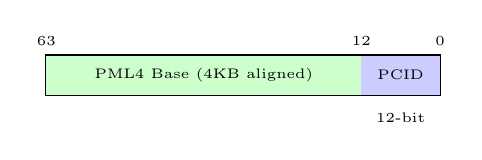
\begin{tikzpicture}
    % CR3 register
    \draw[thick] (0,0) rectangle (5,0.5);
    \fill[green!20] (0,0) rectangle (4,0.5);
    \fill[blue!20] (4,0) rectangle (5,0.5);

    % Bit positions
    \node[above, font=\tiny] at (0,0.5) {63};
    \node[above, font=\tiny] at (4,0.5) {12};
    \node[above, font=\tiny] at (5,0.5) {0};

    % Labels
    \node[font=\tiny] at (2,0.25) {PML4 Base (4KB aligned)};
    \node[font=\tiny] at (4.5,0.25) {PCID};

    % PCID note
    \node[below, font=\tiny] at (4.5,-0.1) {12-bit};
\end{tikzpicture}
\end{center}

\textbf{ARM: ASID in TTBR0\_EL1}
\begin{itemize}
\item 8-bit or 16-bit ASID field
\end{itemize}
\end{column}
\end{columns}
\end{frame}

\begin{frame}{ASID: Practical Limitations}
\begin{columns}[T]
\begin{column}{0.5\textwidth}
\textbf{Limited ASID space:}
\begin{itemize}
\item x86: $2^{12}$ = 4096 PCIDs
\item ARM: $2^{8}$ = 256 or $2^{16}$ = 65536 ASIDs
\item Not enough for all processes on busy systems
\item OS must manage ASID allocation/recycling
\item ASID reuse $\rightarrow$ selective TLB flush needed
\end{itemize}
\end{column}

\begin{column}{0.5\textwidth}
\textbf{TLB implementation constraints:}
\begin{itemize}
\item TLBs may store fewer ASID bits than arch defines
\item Some TLBs hash the ASID $\rightarrow$ collisions
\item Causes ``ASID aliasing'': unrelated processes evict each other's entries
\item Different TLB levels may have different ASID support
\end{itemize}
\end{column}
\end{columns}
\end{frame}

% Temporarily removed TLB Lookup with ASID frame due to matrix node reference issues
% TODO: Fix the matrix node references or recreate without matrix

\begin{frame}{Contiguous PTE (ContPTE) - ARM Feature}
\begin{columns}[T]
\begin{column}{0.45\textwidth}
\textbf{Problem:} TLB pressure
\begin{itemize}
\item One TLB entry per 4KB page
\item Large regions → many TLB entries
\item 2MB pages often too large
\end{itemize}

\textbf{ContPTE Solution:}
\begin{itemize}
\item 16 consecutive PTEs marked "contiguous"
\item Maps 64KB (16 × 4KB)
\item Hardware coalesces into single TLB entry
\end{itemize}

\textbf{Requirements:}
\begin{itemize}
\item Physical pages must be contiguous
\item Same permissions for all 16 pages
\item Contiguous bit set in all 16 PTEs
\end{itemize}

\textbf{Benefits:}
\begin{itemize}
\item 16× TLB reach improvement
\item No page table format changes
\item Transparent to applications
\end{itemize}
\end{column}

\begin{column}{0.55\textwidth}
\vspace{-5mm}
\begin{center}
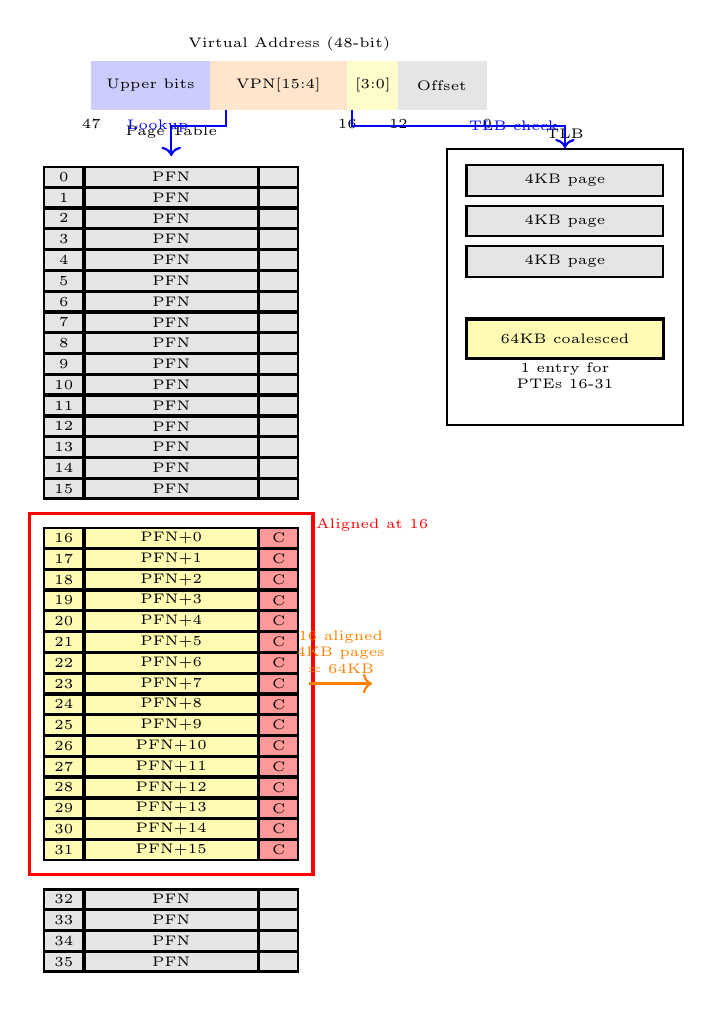
\begin{tikzpicture}[
    pte cell/.style={draw, thick, minimum height=2.5mm, font=\tiny, inner sep=1pt, anchor=center},
    idx cell/.style={pte cell, minimum width=5mm},
    pfn cell/.style={pte cell, minimum width=22mm},
    flag cell/.style={pte cell, minimum width=5mm},
    tlb_entry/.style={draw, thick, minimum width=25mm, minimum height=3.5mm, font=\tiny},
    section_title/.style={font=\tiny, anchor=south}
]
    % Virtual Address at top (style from TLB Lookup slide)
    \node[draw, thick, minimum width=50mm, minimum height=6mm, inner sep=0pt] (va) at (0,0) {};
    \node[above, font=\tiny] at (va.north) {Virtual Address (48-bit)};

    % VA fields
    \fill[blue!20] (va.north west) rectangle ([xshift=15mm]va.south west);
    \fill[orange!20] ([xshift=15mm]va.north west) rectangle ([xshift=32.5mm]va.south west);
    \fill[yellow!20] ([xshift=32.5mm]va.north west) rectangle ([xshift=39mm]va.south west);
    \fill[gray!20] ([xshift=39mm]va.north west) rectangle (va.south east);

    \node[font=\tiny] at ([xshift=7.5mm]va.west) {Upper bits};
    \node[font=\tiny] at ([xshift=23.75mm]va.west) {VPN[15:4]};
    \node[font=\tiny] at ([xshift=35.75mm]va.west) {[3:0]};
    \node[font=\tiny] at ([xshift=44.5mm]va.west) {Offset};

    % Bit positions
    \node[below, font=\tiny] at (va.south west) {47};
    \node[below, font=\tiny] at ([xshift=32.5mm]va.south west) {16};
    \node[below, font=\tiny] at ([xshift=39mm]va.south west) {12};
    \node[below, font=\tiny] at (va.south east) {0};

    % Page table title
    \node[section_title] (pt_title) at (-1.5,-0.8) {Page Table};

    % Regular PTEs (0-15) using matrix
    \matrix[matrix of nodes,
        anchor=north,
        row sep=-\pgflinewidth,
        column sep=-\pgflinewidth,
        ampersand replacement=\&,
        nodes={pte cell, fill=gray!20},
        column 1/.style={nodes={idx cell}},
        column 2/.style={nodes={pfn cell}},
        column 3/.style={nodes={flag cell}},
    ] (pte_reg) at ([yshift=-1mm]pt_title.south) {
        0 \& PFN \& {} \\
        1 \& PFN \& {} \\
        2 \& PFN \& {} \\
        3 \& PFN \& {} \\
        4 \& PFN \& {} \\
        5 \& PFN \& {} \\
        6 \& PFN \& {} \\
        7 \& PFN \& {} \\
        8 \& PFN \& {} \\
        9 \& PFN \& {} \\
        10 \& PFN \& {} \\
        11 \& PFN \& {} \\
        12 \& PFN \& {} \\
        13 \& PFN \& {} \\
        14 \& PFN \& {} \\
        15 \& PFN \& {} \\
    };

    % Contiguous PTEs (16-31) using matrix
    \matrix[matrix of nodes,
        anchor=north,
        row sep=-\pgflinewidth,
        column sep=-\pgflinewidth,
        ampersand replacement=\&,
        nodes={pte cell, fill=yellow!30},
        column 1/.style={nodes={idx cell}},
        column 2/.style={nodes={pfn cell}},
        column 3/.style={nodes={flag cell, fill=red!40}},
    ] (pte_contig) at ([yshift=-1mm]pte_reg.south) {
        16 \& PFN+0 \& C \\
        17 \& PFN+1 \& C \\
        18 \& PFN+2 \& C \\
        19 \& PFN+3 \& C \\
        20 \& PFN+4 \& C \\
        21 \& PFN+5 \& C \\
        22 \& PFN+6 \& C \\
        23 \& PFN+7 \& C \\
        24 \& PFN+8 \& C \\
        25 \& PFN+9 \& C \\
        26 \& PFN+10 \& C \\
        27 \& PFN+11 \& C \\
        28 \& PFN+12 \& C \\
        29 \& PFN+13 \& C \\
        30 \& PFN+14 \& C \\
        31 \& PFN+15 \& C \\
    };

    % Red border around contiguous block
    \draw[thick, red, line width=1.2pt]
        ([shift={(-0.5mm,0.5mm)}]pte_contig.north west) rectangle
        ([shift={(0.5mm,-0.5mm)}]pte_contig.south east);

    % More regular PTEs (32+) using matrix
    \matrix[matrix of nodes,
        anchor=north,
        row sep=-\pgflinewidth,
        column sep=-\pgflinewidth,
        ampersand replacement=\&,
        nodes={pte cell, fill=gray!20},
        column 1/.style={nodes={idx cell}},
        column 2/.style={nodes={pfn cell}},
        column 3/.style={nodes={flag cell}},
    ] (pte_more) at ([yshift=-1mm]pte_contig.south) {
        32 \& PFN \& {} \\
        33 \& PFN \& {} \\
        34 \& PFN \& {} \\
        35 \& PFN \& {} \\
    };

    % Arrow with label for contiguous block
    \draw[->, thick, orange] (pte_contig.east |- pte_contig-8-1) -- ++(8mm,0)
        node[midway, above, font=\tiny, align=center] {16 aligned\\4KB pages\\= 64KB};
    \node[font=\tiny, red] at ([xshift=8mm, yshift=-1mm]pte_contig.north east) {Aligned at 16};

    % TLB
    \node[section_title] (tlb_title) at (3.5,-0.8) {TLB};

    % TLB box
    \node[draw, thick, minimum width=30mm, minimum height=35mm, anchor=north] (tlb_box) at (tlb_title.south) {};

    % Regular TLB entries
    \node[tlb_entry, fill=gray!20, anchor=north] (tlb0) at ([yshift=-2mm]tlb_title.south) {4KB page};
    \node[tlb_entry, fill=gray!20, anchor=north] (tlb1) at ([yshift=-1mm]tlb0.south) {4KB page};
    \node[tlb_entry, fill=gray!20, anchor=north] (tlb2) at ([yshift=-1mm]tlb1.south) {4KB page};

    % Coalesced entry (emphasized)
    \node[tlb_entry, fill=yellow!30, line width=1.2pt, minimum height=5mm, anchor=north]
        (tlb_coal) at ([yshift=-5mm]tlb2.south) {64KB coalesced};

    % Annotation
    \node[font=\tiny, align=center] at ([yshift=-2mm]tlb_coal.south) {1 entry for\\PTEs 16-31};

    % Lookup arrows from VA to Page Table and TLB
    \draw[->, thick, blue] ([xshift=-8mm]va.south) -- ++(0,-2mm) -| (pte_reg.north)
        node[pos=0.25, left, font=\tiny] {Lookup};
    \draw[->, thick, blue] ([xshift=8mm]va.south) -- ++(0,-2mm) -| (tlb_box.north)
        node[pos=0.25, right, font=\tiny] {TLB check};
\end{tikzpicture}
\end{center}
\end{column}
\end{columns}
\end{frame}

\begin{frame}{ContPTE: TLB Lookup Mechanism}
\begin{center}
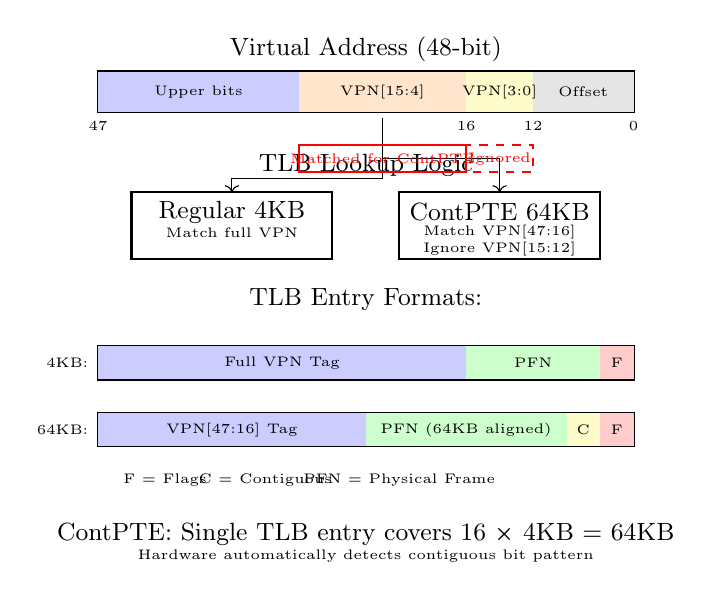
\begin{tikzpicture}[scale=0.85]
    % Virtual Address
    \draw[thick] (0,6) rectangle (8,6.6);
    \node[above, font=\small] at (4,6.6) {Virtual Address (48-bit)};
    
    % VA fields
    \fill[blue!20] (0,6) rectangle (3,6.6);
    \fill[orange!20] (3,6) rectangle (5.5,6.6);
    \fill[yellow!20] (5.5,6) rectangle (6.5,6.6);
    \fill[gray!20] (6.5,6) rectangle (8,6.6);
    
    \node[font=\tiny] at (1.5,6.3) {Upper bits};
    \node[font=\tiny] at (4.25,6.3) {VPN[15:4]};
    \node[font=\tiny] at (6,6.3) {VPN[3:0]};
    \node[font=\tiny] at (7.25,6.3) {Offset};
    
    % Bit positions
    \node[below, font=\tiny] at (0,6) {47};
    \node[below, font=\tiny] at (5.5,6) {16};
    \node[below, font=\tiny] at (6.5,6) {12};
    \node[below, font=\tiny] at (8,6) {0};
    
    % TLB lookup paths
    \node[font=\small] at (4,5.2) {TLB Lookup Logic};
    
    % Regular 4KB lookup
    \draw[thick] (0.5,4.8) rectangle (3.5,3.8);
    \node[font=\small] at (2,4.5) {Regular 4KB};
    \node[font=\tiny] at (2,4.2) {Match full VPN};
    \draw[->] (4.25,5.9) -- (4.25,5) -- (2,5) -- (2,4.8);
    
    % ContPTE 64KB lookup
    \draw[thick] (4.5,4.8) rectangle (7.5,3.8);
    \node[font=\small] at (6,4.5) {ContPTE 64KB};
    \node[font=\tiny] at (6,4.2) {Match VPN[47:16]};
    \node[font=\tiny] at (6,3.95) {Ignore VPN[15:12]};
    \draw[->] (4.25,5.9) -- (4.25,5.3) -- (6,5.3) -- (6,4.8);
    
    % Show which bits are matched
    \draw[thick, red] (3,5.5) rectangle (5.5,5.1);
    \node[font=\tiny, red] at (4.25,5.3) {Matched for ContPTE};
    
    \draw[thick, dashed, red] (5.5,5.5) rectangle (6.5,5.1);
    \node[font=\tiny, red] at (6,5.3) {Ignored};
    
    % TLB entry format
    \node[font=\small] at (4,3.2) {TLB Entry Formats:};
    
    % 4KB entry
    \draw[thick] (0,2.5) rectangle (8,2);
    \fill[blue!20] (0,2.5) rectangle (5.5,2);
    \fill[green!20] (5.5,2.5) rectangle (7.5,2);
    \fill[red!20] (7.5,2.5) rectangle (8,2);
    \node[font=\tiny] at (2.75,2.25) {Full VPN Tag};
    \node[font=\tiny] at (6.5,2.25) {PFN};
    \node[font=\tiny] at (7.75,2.25) {F};
    \node[left, font=\tiny] at (0,2.25) {4KB:};
    
    % 64KB entry
    \draw[thick] (0,1.5) rectangle (8,1);
    \fill[blue!20] (0,1.5) rectangle (4,1);
    \fill[green!20] (4,1.5) rectangle (7,1);
    \fill[yellow!20] (7,1.5) rectangle (7.5,1);
    \fill[red!20] (7.5,1.5) rectangle (8,1);
    \node[font=\tiny] at (2,1.25) {VPN[47:16] Tag};
    \node[font=\tiny] at (5.5,1.25) {PFN (64KB aligned)};
    \node[font=\tiny] at (7.25,1.25) {C};
    \node[font=\tiny] at (7.75,1.25) {F};
    \node[left, font=\tiny] at (0,1.25) {64KB:};
    
    % Legend
    \node[font=\tiny] at (1,0.5) {F = Flags};
    \node[font=\tiny] at (2.5,0.5) {C = Contiguous};
    \node[font=\tiny] at (4.5,0.5) {PFN = Physical Frame};
    
    % Bottom note
    \node[below, font=\small, align=center] at (4,0) {ContPTE: Single TLB entry covers 16 × 4KB = 64KB};
    \node[below, font=\tiny, align=center] at (4,-0.4) {Hardware automatically detects contiguous bit pattern};
\end{tikzpicture}
\end{center}
\end{frame}

\begin{frame}{TLB Shootdown: Maintaining Coherency}
\begin{columns}[T]
\begin{column}{0.6\textwidth}
\textbf{Problem: TLB coherency across cores}
\begin{itemize}
\item CPU 0 unmaps a page
\item CPU 1's TLB still has old mapping
\item Can access freed/reused memory!
\end{itemize}

\textbf{Classic TLB Shootdown (IPI-based):}
\begin{enumerate}
\item Initiator updates page table
\item Send Inter-Processor Interrupt to all CPUs
\item Each CPU runs \textbf{software handler} to invalidate TLB
\item CPUs signal completion via \textbf{memory write} (ACK)
\item Initiator polls/waits, then continues
\end{enumerate}

\textbf{Performance impact:}
\begin{itemize}
\item Synchronous operation - initiator waits
\item IPIs interrupt all CPUs (context switch overhead)
\item Scales poorly with core count
\end{itemize}

\textbf{Software optimizations possible:}
\begin{itemize}
\item Batch multiple invalidations
\item Selective targeting (skip idle CPUs)
\item Lazy TLB mode for kernel threads
\end{itemize}
\end{column}

\begin{column}{0.4\textwidth}
\begin{center}
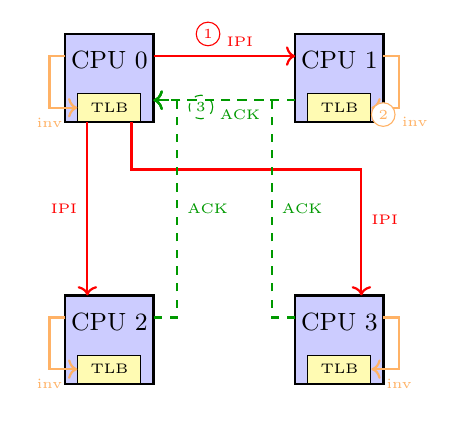
\begin{tikzpicture}[
    % CPU style - symmetric pins (NL=NR, NT=NB)
    cpublock/.style={muxdemux, muxdemux def={NL=2, NR=2, NT=2, NB=2, Lh=2, Rh=2, w=2},
        external pins width=0, fill=blue!20},
    % TLB style - narrower than CPU, anchored at north to CPU's south
    tlbbox/.style={rectangle, draw, minimum width=0.8cm, minimum height=0.3cm,
        fill=yellow!30, font=\tiny, anchor=south},
    % Label style
    lbl/.style={font=\tiny},
    % CPU label style - positioned at top of CPU
    cpulbl/.style={font=\small, anchor=north},
    % Circled number style
    stepnum/.style={circle, draw, fill=white, font=\tiny, inner sep=1pt, minimum size=3mm}
]
    % CPU 0 (top-left) - reference node
    \node[cpublock] (cpu0) {};
    \node[cpulbl] at ([yshift=-1mm]cpu0.north) {CPU 0};
    \node[tlbbox] (tlb0) at (cpu0.south) {TLB};

    % CPU 1 (top-right) - relative to CPU 0
    \node[cpublock, right=18mm of cpu0] (cpu1) {};
    \node[cpulbl] at ([yshift=-1mm]cpu1.north) {CPU 1};
    \node[tlbbox] (tlb1) at (cpu1.south) {TLB};

    % CPU 2 (bottom-left) - relative to CPU 0
    \node[cpublock, below=22mm of cpu0] (cpu2) {};
    \node[cpulbl] at ([yshift=-1mm]cpu2.north) {CPU 2};
    \node[tlbbox] (tlb2) at (cpu2.south) {TLB};

    % CPU 3 (bottom-right) - relative to CPU 1
    \node[cpublock, below=22mm of cpu1] (cpu3) {};
    \node[cpulbl] at ([yshift=-1mm]cpu3.north) {CPU 3};
    \node[tlbbox] (tlb3) at (cpu3.south) {TLB};

    % IPI arrows from CPU 0 (red, solid)
    % CPU0 → CPU1: straight horizontal
    \draw[->, thick, red] (cpu0.rpin 1) -- node[lbl, above] {\raisebox{0pt}[0pt][0pt]{\tikz\node[stepnum]{1};} IPI} (cpu1.lpin 1);
    % CPU0 → CPU2: straight vertical
    \draw[->, thick, red] (cpu0.bpin 1) -- node[lbl, left] {IPI} (cpu2.tpin 1);
    % CPU0 → CPU3: routed diagonal
    \draw[->, thick, red] (cpu0.bpin 2) -- ++(0,-6mm) -| node[lbl, pos=0.7, right] {IPI} (cpu3.tpin 2);

    % ACK arrows back to CPU 0 - all to rpin 2
    \draw[->, thick, dashed, green!60!black] (cpu1.lpin 2) -- node[lbl, below] {\raisebox{0pt}[0pt][0pt]{\tikz\node[stepnum]{3};} ACK} (cpu0.rpin 2);
    \draw[->, thick, dashed, green!60!black] (cpu2.rpin 1) -- ++(3mm,0) |- node[lbl, pos=0.25, right] {ACK} (cpu0.rpin 2);
    \draw[->, thick, dashed, green!60!black] (cpu3.lpin 1) -- ++(-3mm,0) |- node[lbl, pos=0.25, right] {ACK} (cpu0.rpin 2);

    % Local TLB invalidation: left CPUs from lpin to TLB west, right CPUs from rpin to TLB east
    \draw[->, thick, orange!60] (cpu0.lpin 1) -- ++(-2mm,0) |- node[lbl, below] {inv} (tlb0.west);
    \draw[->, thick, orange!60] (cpu1.rpin 1) -- ++(2mm,0) |- node[lbl, below] {\raisebox{0pt}[0pt][0pt]{\tikz\node[stepnum]{2};} inv} (tlb1.east);
    \draw[->, thick, orange!60] (cpu2.lpin 1) -- ++(-2mm,0) |- node[lbl, below] {inv} (tlb2.west);
    \draw[->, thick, orange!60] (cpu3.rpin 1) -- ++(2mm,0) |- node[lbl, below] {inv} (tlb3.east);
\end{tikzpicture}
\end{center}
\end{column}
\end{columns}
\end{frame}

\begin{frame}{Modern TLB Invalidation: Broadcast Instructions}
\begin{columns}[T]
\begin{column}{0.5\textwidth}
\textbf{INVLPGB (AMD) / TLBSYNC:}
\begin{itemize}
\item Broadcast invalidation without IPIs
\item Hardware handles coherency protocol
\item Non-blocking for initiator
\end{itemize}

\textbf{How it works:}
\begin{enumerate}
\item Execute INVLPGB with address range
\item Hardware broadcasts to all cores
\item TLBSYNC waits for completion
\item Can continue other work between INVLPGB and TLBSYNC
\end{enumerate}

\textbf{ARM: TLBI with broadcast}
\begin{itemize}
\item TLBI instructions with Inner Shareable scope
\item Automatic broadcast to all cores in domain
\item No software IPIs needed
\end{itemize}
\end{column}

\begin{column}{0.5\textwidth}
\textbf{Benefits:}
\begin{itemize}
\item No IPI overhead (no context switches)
\item Better scalability with core count
\item Asynchronous operation possible
\item Lower latency for munmap(), mprotect()
\end{itemize}

\textbf{Limitations:}
\begin{itemize}
\item \textbf{All-or-nothing}: cannot skip idle CPUs
\item Only options: all cores or local-only
\item Software IPIs allow selective targeting
\item Limited ASID bits (8-16) $\rightarrow$ ASID reuse requires global flush, negating broadcast benefits
\end{itemize}

\textbf{When broadcast wins:}
\begin{itemize}
\item JVM garbage collectors (unmapping large heaps)
\item Database buffer pool resizing
\item Container memory limit changes
\item High core count systems (>32 cores)
\end{itemize}
\end{column}
\end{columns}
\end{frame}

\begin{frame}{Software Impact: When These Features Matter}
\begin{itemize}
\item \textbf{ASID helps when:}
    \begin{itemize}
    \item Many short-lived processes (web servers, shell scripts)
    \item Frequent system calls with KPTI/Meltdown mitigation
    \item Container workloads with namespace switches
    \end{itemize}
    
\item \textbf{ContPTE/THP benefits:}
    \begin{itemize}
    \item Large memory allocations (databases, scientific computing)
    \item Better than nothing when huge pages fragment
    \item mmap() with MAP\_POPULATE for large files
    \end{itemize}
    
\item \textbf{TLB shootdown overhead visible in:}
    \begin{itemize}
    \item fork()/exit() in multithreaded programs
    \item Memory-mapped file operations across threads
    \item Dynamic memory allocators (malloc/free of large chunks)
    \item Live migration of VMs
    \end{itemize}
    
\item \textbf{Performance monitoring:}
    \begin{itemize}
    \item \texttt{perf stat -e tlb:tlb\_flush} - count TLB flushes
    \item \texttt{/proc/interrupts} - look for TLB shootdown IPIs
    \item High system CPU time often indicates TLB management overhead
    \end{itemize}
\end{itemize}
\end{frame}

% Backup slides section
\section{Backup}

\begin{frame}{Backup}
\begin{center}
\Huge Backup
\end{center}
\end{frame}

\begin{frame}{Why Virtual Memory?}
\begin{itemize}
\item \textbf{Generality} – ability to run programs larger than size of physical memory
\item \textbf{Storage management} – allocation/deallocation of variable sized blocks is costly and leads to (external) fragmentation
\item \textbf{Protection} – regions of the address space can be R/O, Ex, ...
\item \textbf{Flexibility} – portions of a program can be placed anywhere, without relocation
\item \textbf{Storage efficiency} – retain only most important portions of the program in memory
\item \textbf{Concurrent I/O} – execute other processes while loading/dumping page
\item \textbf{Expandability} – can leave room in virtual address space for objects to grow
\item \textbf{Performance}
\end{itemize}
\end{frame}

\begin{frame}{Page Aliasing}
\textbf{OS may map different virtual pages to the same physical page}

\textbf{DLLs in Linux/Windows}
\begin{itemize}
\item DLL pages are used by all processes, marked as read only
\item Same DLL may be loaded by a process more than once
\end{itemize}

\textbf{Large malloc – Copy-on-Write}
\begin{itemize}
\item OS maps all allocated virtual pages to the same all-zero physical page
\item The newly allocated virtual page is marked as read-only in its PTE
\item In case of a write to one of these virtual pages:
    \begin{itemize}
    \item Get access violation page-fault
    \item OS identifies that the page is mapped to the special physical page
    \item OS allocates a "real" physical page (copy-on-write)
    \end{itemize}
\end{itemize}

\textbf{Shared Memory}
\begin{itemize}
\item OS maps virtual pages of different processes to the same physical page
\end{itemize}
\end{frame}

\begin{frame}{32bit Mode: 4KB Page Mapping}
\textbf{2-level hierarchical mapping}
\begin{itemize}
\item Page directory and page tables
\item Pages / page tables are 4KB aligned
\end{itemize}

\begin{itemize}
\item CR3 points to the current Page Directory
\item Upper 10 Linear addr. bits point to a PDE
    \begin{itemize}
    \item PDE provides a 20 bit, 4KB aligned base physical address of a page table
    \end{itemize}
\item Next 10 Linear addr. bits point to a PTE within the given Page Table
    \begin{itemize}
    \item PTE provides a 20 bit, 4KB aligned, base physical address of a 4KB page
    \end{itemize}
\item Lowest 12 Linear Addr. bits provide offset within the selected 4KB page
\end{itemize}
\end{frame}

\begin{frame}{32bit Mode: 4MB Page Mapping}
\begin{itemize}
\item PDE directly maps up to 1024 4MB pages
\item Upper 10 Linear addr. bits point to a PDE
    \begin{itemize}
    \item PS in the PDE = 1
    \item PDE provides a 10 bit, 4MB aligned, base physical address of a 4MB page
    \end{itemize}
\item Lowest 22 Linear addr. bits provide offset within selected 4MB page
\end{itemize}

\textbf{Mixing 4KByte and 4MByte Pages}
\begin{itemize}
\item Separate TLBs for 4MB pages and 4KB pages
    \begin{itemize}
    \item Often-used code (e.g., kernels) is placed in a 4MB page $\rightarrow$ frees up 4KB TLB entries
    \item Reduces TLB misses and improve overall system performance
    \end{itemize}
\end{itemize}
\end{frame}

\begin{frame}{PAE – Physical Address Extension}
\textbf{When PAE (physical address extension) flag in CR4 is set}
\begin{itemize}
\item Physical addresses is extended to M bits
    \begin{itemize}
    \item Linear address remains 32 bit
    \end{itemize}
\item Each page table entry becomes 64 bits to hold the extra phy. address bits
    \begin{itemize}
    \item Page directory and page tables remain 4KB in size
    \item Number of entries in each table is halved to 512
    \item Indexed by 9 instead of 10 bits
    \end{itemize}
\end{itemize}

\textbf{A new 4 entry Page Directory Pointer Table is added}
\begin{itemize}
\item Indexed by bits [31:30] of the linear address
\item Each entry points to a page directory
\item CR3 contains the page-directory-pointer-table base address
    \begin{itemize}
    \item Provides the m.s.bits of the physical address
    \item Forcing the table to be located on a 32-byte boundary
    \end{itemize}
\end{itemize}
\end{frame}

\begin{frame}{Execute-Disable Bit}
\textbf{Supported only with PAE enabled / 64 bit mode}
\begin{itemize}
\item Bit[63] in PML4 entry, PDP entry, PDE, PTE
\end{itemize}

\textbf{If the execute disable bit of a memory page is set}
\begin{itemize}
\item The page can be used only as data
\item An attempt to execute code from a memory page with the execute-disable bit set causes a page-fault exception
\item Setting the execute-disable bit at any level of the paging structure, protects all pages pointed from this entry
\end{itemize}
\end{frame}

\begin{frame}{Page Table – Virtual Mem. Attributes}
\textbf{Present (P) flag}
\begin{itemize}
\item When set: page is in physical memory
\item When clear, page not in memory $\rightarrow$ processor generates a page-fault
\item The processor does not set/clear this flag – OS maintains its state
\item In case of a page-fault, the OS performs the following operations:
    \begin{enumerate}
    \item Copy the page from disk into physical memory
    \item Load page address into PTE/PDE; set present=1, dirty=0, accessed=0
    \item Invalidate victim page from TLB
    \item Return from page-fault handler and restart the program
    \end{enumerate}
\end{itemize}

\textbf{Page size (PS) flag, in PDEs only}
\begin{itemize}
\item 0: The PDE points to a page table of 4KBytes pages
\item 1: The PDE points to a 4MB page
\end{itemize}
\end{frame}

\begin{frame}{Page Table – Virtual Mem. Attributes (cont.)}
\textbf{Accessed (A) flag and Dirty (D) flag}
\begin{itemize}
\item Typically cleared by the OS when a page/PT initially loaded into physical mem
\item Processor sets the A-flag the first time a page/PT is accessed (read/write)
\item Processor sets the D-flag the first time a page is accessed for a write
    \begin{itemize}
    \item The D-flag is not used in PDEs which point to page tables
    \end{itemize}
\item Both A and D flag are sticky
    \begin{itemize}
    \item Once set, the processor does not implicitly clear it – only software can clear it
    \end{itemize}
\item Used by OS to manage transfer of pages/PTs tables into and out of physical memory
\end{itemize}

\textbf{Global (G) flag}
\begin{itemize}
\item Indicates a global page when set (+ page global enable is set: CR4.PGE =1)
\item PTE/PDE in TLB not invalidated when CR3 is loaded / task switch
\item Only software can set or clear this flag
\end{itemize}
\end{frame}

\begin{frame}{Page Table – Caching Attributes}
\textbf{Page-level write-through (PWT) flag}
\begin{itemize}
\item Controls the write-through or write-back caching policy of the page / PT
    \begin{itemize}
    \item 0 : write-back caching, 1: write-through caching
    \end{itemize}
\item Ignored if the CD (cache disable) flag in CR0 is set
\end{itemize}

\textbf{Page-level cache disable (PCD) flag}
\begin{itemize}
\item Controls the caching of individual pages/PT
\item 1: caching of the associated page/PT is prevented
\item 0: the page/PT can be cached
\item Ignored (assumes as set) if the CD (cache disable) flag in CR0 is set
\end{itemize}

\textbf{Page table attribute index (PAT) flag}
\begin{itemize}
\item Used along with the PCD and PWT flags to select an entry in the PAT
\item Which in turn selects the memory type for the page
\end{itemize}
\end{frame}

\begin{frame}{Page Table – Protection Attributes}
\textbf{Read/write (R/W) flag}
\begin{itemize}
\item Specifies the read-write privileges for a page or group of pages
\item 0: the page is read only
\item 1: the page can be read and written into
\end{itemize}

\textbf{User/supervisor (U/S) flag}
\begin{itemize}
\item Specifies the user-supervisor privileges for a page or group of pages
\item 0: supervisor privilege level
\item 1: user privilege level
\end{itemize}
\end{frame}

\begin{frame}{Page Table Base Register (PTBR)}
\textbf{The physical address of the root page table is stored in a special register}
\begin{itemize}
\item Called the Page Table Base Register (PTBR)
\item In x86-64: CR3 register points to the PML4 table
\item Each process has its own PTBR value
\end{itemize}

\textbf{PTBR is loaded as part of a context switch}

\textbf{OS must ensure that}
\begin{itemize}
\item The root page table pointed to by PTBR is present in physical memory before the process is dispatched
\item The page table hierarchy remains in memory while the process is active
\end{itemize}
\end{frame}

\begin{frame}{TLBs}
\textbf{OS running at privilege level 0 can invalidate TLB entries}
\begin{itemize}
\item INVLPG instruction invalidates a specific PTE in the TLB
    \begin{itemize}
    \item This instruction ignores the setting of the G flag
    \end{itemize}
\item Whenever a PDE/PTE is changed (also when present flag is set to 0)
    \begin{itemize}
    \item OS must invalidate the corresponding TLB entry
    \end{itemize}
\item All (non-global) TLBs are automatically invalidated when CR3 is loaded
\end{itemize}

\textbf{The global (G) flag prevents frequently used pages from being automatically invalidated in on a task switch}
\begin{itemize}
\item The entry remains in the TLB indefinitely
\item Only INVLPG can invalidate a global page entry
\end{itemize}
\end{frame}

\begin{frame}{PTE/PDE/PDP/PML4 Entry Format}
\tiny
\definecolor{addrcolor}{HTML}{E6E6FA}
\definecolor{igncolor}{HTML}{FFE4E1}
\definecolor{rsvcolor}{HTML}{F0F0F0}
\definecolor{pagesizeyellow}{HTML}{FFFF00}

\begin{tikzpicture}[scale=1, transform shape]

% Bit numbers at top
\node[anchor=east] at (0.1,7.6) {\tiny 63};
\node[anchor=west] at (1.8,7.6) {\tiny 52 51};
\node[anchor=center] at (6.0,7.6) {\tiny M M-1};
\node[anchor=east] at (9.3,7.6) {\tiny 12 11};
\node[anchor=east] at (10.5,7.6) {\tiny 9 8 7 6 5 4 3 2 1 0};

% CR3 row
\draw[thick] (0,7.2) rectangle (11.4,6.4);
\fill[rsvcolor] (0,7.2) rectangle (2.1,6.4);
\fill[addrcolor] (2.1,7.2) rectangle (9.4,6.4);
\fill[igncolor] (9.4,7.2) rectangle (10.5,6.4);
\node at (1.05,6.8) {\tiny Reserved};
\node at (5.75,6.8) {\tiny Address of PML4 table};
\node at (9.95,6.8) {\tiny Ignored};
% Draw individual bit cells for flags
\foreach \x in {10.5,10.65,10.8,10.95,11.1,11.25} {
    \draw ({\x},7.2) rectangle ({\x+0.15},6.4);
}
\node[anchor=west] at (11.6,6.8) {\textbf{CR3}};

% PML4E row
\draw[thick] (0,6.4) rectangle (11.4,5.6);
\fill[igncolor] (0,6.4) rectangle (0.3,5.6);
\fill[igncolor] (0.3,6.4) rectangle (2.1,5.6);
\fill[rsvcolor] (2.1,6.4) rectangle (2.7,5.6);
\fill[addrcolor] (2.7,6.4) rectangle (9.4,5.6);
\fill[igncolor] (9.4,6.4) rectangle (9.9,5.6);
\node[rotate=90,anchor=center] at (0.15,6.0) {\tiny XD};
\node at (1.2,6.0) {\tiny Ignored};
\node at (2.4,6.0) {\tiny Rsvd.};
\node at (6.05,6.0) {\tiny Address of page-directory-pointer table};
\node at (9.65,6.0) {\tiny Ign.};
% Individual flag bits
\foreach \x in {9.9,10.05,10.2,10.35,10.5,10.65,10.8,10.95,11.1,11.25} {
    \draw ({\x},6.4) rectangle ({\x+0.15},5.6);
}
\node[rotate=90,anchor=center] at (10.125,6.0) {\tiny A};
\node[rotate=90,anchor=center] at (10.575,6.0) {\tiny PCD};
\node[rotate=90,anchor=center] at (10.725,6.0) {\tiny PWT};
\node[rotate=90,anchor=center] at (10.875,6.0) {\tiny US};
\node[rotate=90,anchor=center] at (11.025,6.0) {\tiny RW};
\node[rotate=90,anchor=center] at (11.175,6.0) {\tiny P};
\node[anchor=west] at (11.6,6.2) {\textbf{PML4E:}};
\node[anchor=west] at (11.6,5.8) {\textbf{present}};

% PDPTE 1GB row
\draw[thick] (0,5.6) rectangle (11.4,4.8);
\fill[igncolor] (0,5.6) rectangle (0.3,4.8);
\fill[igncolor] (0.3,5.6) rectangle (2.1,4.8);
\fill[rsvcolor] (2.1,5.6) rectangle (2.7,4.8);
\fill[addrcolor] (2.7,5.6) rectangle (5.8,4.8);
\fill[rsvcolor] (5.8,5.6) rectangle (9.4,4.8);
\fill[igncolor] (9.4,5.6) rectangle (9.75,4.8);
\node[rotate=90,anchor=center] at (0.15,5.2) {\tiny XD};
\node at (1.2,5.2) {\tiny Ignored};
\node at (2.4,5.2) {\tiny Rsvd.};
\node at (4.25,5.2) {\tiny\begin{tabular}{c}Address of\\1GB page frame\end{tabular}};
\node at (7.6,5.2) {\tiny Reserved};
\node at (9.575,5.2) {\tiny Ign.};
% Individual flag bits
\foreach \x in {9.75,9.9,10.05,10.2,10.35,10.5,10.65,10.8,10.95,11.1,11.25} {
    \draw ({\x},5.6) rectangle ({\x+0.15},4.8);
}
\fill[pagesizeyellow] (10.35,5.6) rectangle (10.5,4.8);
\node[rotate=90,anchor=center] at (9.825,5.2) {\tiny G};
\node[rotate=90,anchor=center] at (10.125,5.2) {\tiny DA};
\node[rotate=90,anchor=center] at (10.275,5.2) {\tiny A};
\node[rotate=90,anchor=center] at (10.425,5.2) {\tiny 1};
\node[rotate=90,anchor=center] at (10.575,5.2) {\tiny PCD};
\node[rotate=90,anchor=center] at (10.725,5.2) {\tiny PWT};
\node[rotate=90,anchor=center] at (10.875,5.2) {\tiny US};
\node[rotate=90,anchor=center] at (11.025,5.2) {\tiny RW};
\node[rotate=90,anchor=center] at (11.175,5.2) {\tiny P};
\node[anchor=west] at (11.6,5.4) {\textbf{PDPTE:}};
\node[anchor=west] at (11.6,5.2) {\textbf{1GB}};
\node[anchor=west] at (11.6,5.0) {\textbf{page}};

% PDPTE page directory row
\draw[thick] (0,4.8) rectangle (11.4,4.0);
\fill[igncolor] (0,4.8) rectangle (0.3,4.0);
\fill[igncolor] (0.3,4.8) rectangle (2.1,4.0);
\fill[rsvcolor] (2.1,4.8) rectangle (2.7,4.0);
\fill[addrcolor] (2.7,4.8) rectangle (9.4,4.0);
\fill[igncolor] (9.4,4.8) rectangle (9.9,4.0);
\node[rotate=90,anchor=center] at (0.15,4.4) {\tiny XD};
\node at (1.2,4.4) {\tiny Ignored};
\node at (2.4,4.4) {\tiny Rsvd.};
\node at (6.05,4.4) {\tiny Address of page directory};
\node at (9.65,4.4) {\tiny Ign.};
% Individual flag bits
\foreach \x in {9.9,10.05,10.2,10.35,10.5,10.65,10.8,10.95,11.1,11.25} {
    \draw ({\x},4.8) rectangle ({\x+0.15},4.0);
}
\fill[pagesizeyellow] (10.35,4.8) rectangle (10.5,4.0);
\node[rotate=90,anchor=center] at (10.125,4.4) {\tiny A};
\node[rotate=90,anchor=center] at (10.425,4.4) {\tiny 0};
\node[rotate=90,anchor=center] at (10.575,4.4) {\tiny PCD};
\node[rotate=90,anchor=center] at (10.725,4.4) {\tiny PWT};
\node[rotate=90,anchor=center] at (10.875,4.4) {\tiny US};
\node[rotate=90,anchor=center] at (11.025,4.4) {\tiny RW};
\node[rotate=90,anchor=center] at (11.175,4.4) {\tiny P};
\node[anchor=west] at (11.6,4.6) {\textbf{PDPTE:}};
\node[anchor=west] at (11.6,4.4) {\textbf{page}};
\node[anchor=west] at (11.6,4.2) {\textbf{directory}};

% PDE 2MB row
\draw[thick] (0,4.0) rectangle (11.4,3.2);
\fill[igncolor] (0,4.0) rectangle (0.3,3.2);
\fill[igncolor] (0.3,4.0) rectangle (2.1,3.2);
\fill[rsvcolor] (2.1,4.0) rectangle (2.7,3.2);
\fill[addrcolor] (2.7,4.0) rectangle (5.8,3.2);
\fill[rsvcolor] (5.8,4.0) rectangle (9.4,3.2);
\fill[igncolor] (9.4,4.0) rectangle (9.75,3.2);
\node[rotate=90,anchor=center] at (0.15,3.6) {\tiny XD};
\node at (1.2,3.6) {\tiny Ignored};
\node at (2.4,3.6) {\tiny Rsvd.};
\node at (4.25,3.6) {\tiny\begin{tabular}{c}Address of\\2MB page frame\end{tabular}};
\node at (7.6,3.6) {\tiny Reserved};
\node at (9.575,3.6) {\tiny Ign.};
% Individual flag bits
\foreach \x in {9.75,9.9,10.05,10.2,10.35,10.5,10.65,10.8,10.95,11.1,11.25} {
    \draw ({\x},4.0) rectangle ({\x+0.15},3.2);
}
\fill[pagesizeyellow] (10.35,4.0) rectangle (10.5,3.2);
\node[rotate=90,anchor=center] at (9.825,3.6) {\tiny G};
\node[rotate=90,anchor=center] at (10.125,3.6) {\tiny DA};
\node[rotate=90,anchor=center] at (10.275,3.6) {\tiny A};
\node[rotate=90,anchor=center] at (10.425,3.6) {\tiny 1};
\node[rotate=90,anchor=center] at (10.575,3.6) {\tiny PCD};
\node[rotate=90,anchor=center] at (10.725,3.6) {\tiny PWT};
\node[rotate=90,anchor=center] at (10.875,3.6) {\tiny US};
\node[rotate=90,anchor=center] at (11.025,3.6) {\tiny RW};
\node[rotate=90,anchor=center] at (11.175,3.6) {\tiny P};
\node[anchor=west] at (11.6,3.8) {\textbf{PDE:}};
\node[anchor=west] at (11.6,3.6) {\textbf{2MB}};
\node[anchor=west] at (11.6,3.4) {\textbf{page}};

% PDE page table row
\draw[thick] (0,3.2) rectangle (11.4,2.4);
\fill[igncolor] (0,3.2) rectangle (0.3,2.4);
\fill[igncolor] (0.3,3.2) rectangle (2.1,2.4);
\fill[rsvcolor] (2.1,3.2) rectangle (2.7,2.4);
\fill[addrcolor] (2.7,3.2) rectangle (9.4,2.4);
\fill[igncolor] (9.4,3.2) rectangle (9.9,2.4);
\node[rotate=90,anchor=center] at (0.15,2.8) {\tiny XD};
\node at (1.2,2.8) {\tiny Ignored};
\node at (2.4,2.8) {\tiny Rsvd.};
\node at (6.05,2.8) {\tiny Address of page table};
\node at (9.65,2.8) {\tiny Ign.};
% Individual flag bits
\foreach \x in {9.9,10.05,10.2,10.35,10.5,10.65,10.8,10.95,11.1,11.25} {
    \draw ({\x},3.2) rectangle ({\x+0.15},2.4);
}
\fill[pagesizeyellow] (10.35,3.2) rectangle (10.5,2.4);
\node[rotate=90,anchor=center] at (10.125,2.8) {\tiny A};
\node[rotate=90,anchor=center] at (10.425,2.8) {\tiny 0};
\node[rotate=90,anchor=center] at (10.575,2.8) {\tiny PCD};
\node[rotate=90,anchor=center] at (10.725,2.8) {\tiny PWT};
\node[rotate=90,anchor=center] at (10.875,2.8) {\tiny US};
\node[rotate=90,anchor=center] at (11.025,2.8) {\tiny RW};
\node[rotate=90,anchor=center] at (11.175,2.8) {\tiny P};
\node[anchor=west] at (11.6,3.0) {\textbf{PDE:}};
\node[anchor=west] at (11.6,2.8) {\textbf{page}};
\node[anchor=west] at (11.6,2.6) {\textbf{table}};

% PTE row
\draw[thick] (0,2.4) rectangle (11.4,1.6);
\fill[igncolor] (0,2.4) rectangle (0.3,1.6);
\fill[igncolor] (0.3,2.4) rectangle (2.1,1.6);
\fill[rsvcolor] (2.1,2.4) rectangle (2.7,1.6);
\fill[addrcolor] (2.7,2.4) rectangle (9.4,1.6);
\fill[igncolor] (9.4,2.4) rectangle (9.75,1.6);
\node[rotate=90,anchor=center] at (0.15,2.0) {\tiny XD};
\node at (1.2,2.0) {\tiny Ignored};
\node at (2.4,2.0) {\tiny Rsvd.};
\node at (6.05,2.0) {\tiny Address of 4KB page frame};
\node at (9.575,2.0) {\tiny Ign.};
% Individual flag bits
\foreach \x in {9.75,9.9,10.05,10.2,10.35,10.5,10.65,10.8,10.95,11.1,11.25} {
    \draw ({\x},2.4) rectangle ({\x+0.15},1.6);
}
\tiny
\node[rotate=90,anchor=center] at (9.825,2.0) {\tiny G};
\node[rotate=90,anchor=center] at (9.975,2.0) {\tiny PAT};
\node[rotate=90,anchor=center] at (10.125,2.0) {\tiny DA};
\node[rotate=90,anchor=center] at (10.275,2.0) {\tiny A};
\node[rotate=90,anchor=center] at (10.575,2.0) {\tiny PCD};
\node[rotate=90,anchor=center] at (10.725,2.0) {\tiny PWT};
\node[rotate=90,anchor=center] at (10.875,2.0) {\tiny US};
\node[rotate=90,anchor=center] at (11.025,2.0) {\tiny RW};
\node[rotate=90,anchor=center] at (11.175,2.0) {\tiny P};
\node[anchor=west] at (11.6,2.2) {\textbf{PTE:}};
\node[anchor=west] at (11.6,2.0) {\textbf{4KB}};
\node[anchor=west] at (11.6,1.8) {\textbf{page}};

\end{tikzpicture}
\end{frame}


\begin{frame}{PTE/PDE/PDP/PML4 Entry Format}

\definecolor{addrcolor}{HTML}{E6E6FA}
\definecolor{igncolor}{HTML}{FFE4E1}
\definecolor{rsvcolor}{HTML}{F0F0F0}
\definecolor{pagesizeyellow}{HTML}{FFFF00}

\begin{columns}[T]
\begin{column}{0.25\textwidth}
\vspace{-0.5em}
\tiny
\begin{itemize}\setlength{\itemsep}{0.1em}
\item \textbf{Physical frame address}
\item \textbf{Virtual memory}
  \item[] Present -- page is mapped to phys. mem
  \item[] Accessed -- page data was accessed  
  \item[] Dirty -- data in page was modified
  \item[] Global -- remains in TLB on context sw.
  \item[] Page size -- in hierarchies 2 and up
\item \textbf{Protection}
  \item[] R\#/W -- page is read only / writable
  \item[] User / Supervisor\# -- page can be accessed by user+OS or by OS only
  \item[] eXecute Disable -- page can be used only as data (fault if trying to execute)
\item \textbf{Caching}
  \item[] PWT -- Page Write Through
  \item[] PCD -- Page Cache Disabled
  \item[] PAT -- PT Attribute Index
\item \textbf{Ignored} -- bits available for OS usage
\end{itemize}
\end{column}
\begin{column}{0.75\textwidth}
\vspace{-1em}
\setlength{\tabcolsep}{0pt}
\setlength{\fboxsep}{0pt}
\renewcommand{\arraystretch}{1.3}

% Create the main table
\begin{tikzpicture}[scale=0.95, transform shape]

% Bit numbers at top
\node[anchor=east] at (0.1,7.6) {\tiny 63};
\node[anchor=west] at (1.8,7.6) {\tiny 52 51};
\node[anchor=center] at (6.0,7.6) {\tiny M M-1};
\node[anchor=east] at (9.3,7.6) {\tiny 12 11};
\node[anchor=east] at (10.5,7.6) {\tiny 9 8 7 6 5 4 3 2 1 0};

% CR3 row
\draw[thick] (0,7.2) rectangle (11.4,6.4);
\fill[rsvcolor] (0,7.2) rectangle (2.1,6.4);
\fill[addrcolor] (2.1,7.2) rectangle (9.4,6.4);
\fill[igncolor] (9.4,7.2) rectangle (10.5,6.4);
\node at (1.05,6.8) {\tiny Reserved};
\node at (5.75,6.8) {\tiny Address of PML4 table};
\node at (9.95,6.8) {\tiny Ignored};
% Draw individual bit cells for flags
\foreach \x in {10.5,10.65,10.8,10.95,11.1,11.25} {
    \draw ({\x},7.2) rectangle ({\x+0.15},6.4);
}
\node[anchor=west] at (11.6,6.8) {\textbf{CR3}};

% PML4E row
\draw[thick] (0,6.4) rectangle (11.4,5.6);
\fill[igncolor] (0,6.4) rectangle (0.3,5.6);
\fill[igncolor] (0.3,6.4) rectangle (2.1,5.6);
\fill[rsvcolor] (2.1,6.4) rectangle (2.7,5.6);
\fill[addrcolor] (2.7,6.4) rectangle (9.4,5.6);
\fill[igncolor] (9.4,6.4) rectangle (9.9,5.6);
\node[rotate=90,anchor=center] at (0.15,6.0) {\tiny XD};
\node at (1.2,6.0) {\tiny Ignored};
\node at (2.4,6.0) {\tiny Rsvd.};
\node at (6.05,6.0) {\tiny Address of page-directory-pointer table};
\node at (9.65,6.0) {\tiny Ign.};
% Individual flag bits
\foreach \x in {9.9,10.05,10.2,10.35,10.5,10.65,10.8,10.95,11.1,11.25} {
    \draw ({\x},6.4) rectangle ({\x+0.15},5.6);
}
\tiny
\node[rotate=90,anchor=center] at (10.125,6.0) {\tiny A};
\node[rotate=90,anchor=center] at (10.575,6.0) {\tiny PCD};
\node[rotate=90,anchor=center] at (10.725,6.0) {\tiny PWT};
\node[rotate=90,anchor=center] at (10.875,6.0) {\tiny US};
\node[rotate=90,anchor=center] at (11.025,6.0) {\tiny RW};
\node[rotate=90,anchor=center] at (11.175,6.0) {\tiny P};
\node[anchor=west] at (11.6,6.2) {\tiny\textbf{PML4E:}};
\node[anchor=west] at (11.6,5.8) {\tiny\textbf{present}};

% PDPTE 1GB row
\draw[thick] (0,5.6) rectangle (11.4,4.8);
\fill[igncolor] (0,5.6) rectangle (0.3,4.8);
\fill[igncolor] (0.3,5.6) rectangle (2.1,4.8);
\fill[rsvcolor] (2.1,5.6) rectangle (2.7,4.8);
\fill[addrcolor] (2.7,5.6) rectangle (5.8,4.8);
\fill[rsvcolor] (5.8,5.6) rectangle (9.4,4.8);
\fill[igncolor] (9.4,5.6) rectangle (9.75,4.8);
\node[rotate=90,anchor=center] at (0.15,5.2) {\tiny XD};
\node at (1.2,5.2) {\tiny Ignored};
\node at (2.4,5.2) {\tiny Rsvd.};
\node at (4.25,5.2) {\tiny\begin{tabular}{c}Address of\\1GB page frame\end{tabular}};
\node at (7.6,5.2) {\tiny Reserved};
\node at (9.575,5.2) {\tiny Ign.};
% Individual flag bits
\foreach \x in {9.75,9.9,10.05,10.2,10.35,10.5,10.65,10.8,10.95,11.1,11.25} {
    \draw ({\x},5.6) rectangle ({\x+0.15},4.8);
}
\fill[pagesizeyellow] (10.35,5.6) rectangle (10.5,4.8);
\node[rotate=90,anchor=center] at (9.825,5.2) {\tiny G};
\node[rotate=90,anchor=center] at (10.125,5.2) {\tiny DA};
\node[rotate=90,anchor=center] at (10.275,5.2) {\tiny A};
\node[rotate=90,anchor=center] at (10.425,5.2) {\tiny 1};
\node[rotate=90,anchor=center] at (10.575,5.2) {\tiny PCD};
\node[rotate=90,anchor=center] at (10.725,5.2) {\tiny PWT};
\node[rotate=90,anchor=center] at (10.875,5.2) {\tiny US};
\node[rotate=90,anchor=center] at (11.025,5.2) {\tiny RW};
\node[rotate=90,anchor=center] at (11.175,5.2) {\tiny P};
\node[anchor=west] at (11.6,5.4) {\footnotesize\textbf{PDPTE:}};
\node[anchor=west] at (11.6,5.2) {\footnotesize\textbf{1GB}};
\node[anchor=west] at (11.6,5.0) {\footnotesize\textbf{page}};

% PDPTE page directory row
\draw[thick] (0,4.8) rectangle (11.4,4.0);
\fill[igncolor] (0,4.8) rectangle (0.3,4.0);
\fill[igncolor] (0.3,4.8) rectangle (2.1,4.0);
\fill[rsvcolor] (2.1,4.8) rectangle (2.7,4.0);
\fill[addrcolor] (2.7,4.8) rectangle (9.4,4.0);
\fill[igncolor] (9.4,4.8) rectangle (9.9,4.0);
\node[rotate=90,anchor=center] at (0.15,4.4) {\tiny XD};
\node at (1.2,4.4) {\tiny Ignored};
\node at (2.4,4.4) {\tiny Rsvd.};
\node at (6.05,4.4) {\tiny Address of page directory};
\node at (9.65,4.4) {\tiny Ign.};
% Individual flag bits
\foreach \x in {9.9,10.05,10.2,10.35,10.5,10.65,10.8,10.95,11.1,11.25} {
    \draw ({\x},4.8) rectangle ({\x+0.15},4.0);
}
\fill[pagesizeyellow] (10.35,4.8) rectangle (10.5,4.0);
\node[rotate=90,anchor=center] at (10.125,4.4) {\tiny A};
\node[rotate=90,anchor=center] at (10.425,4.4) {\tiny 0};
\node[rotate=90,anchor=center] at (10.575,4.4) {\tiny PCD};
\node[rotate=90,anchor=center] at (10.725,4.4) {\tiny PWT};
\node[rotate=90,anchor=center] at (10.875,4.4) {\tiny US};
\node[rotate=90,anchor=center] at (11.025,4.4) {\tiny RW};
\node[rotate=90,anchor=center] at (11.175,4.4) {\tiny P};
\node[anchor=west] at (11.6,4.6) {\footnotesize\textbf{PDPTE:}};
\node[anchor=west] at (11.6,4.4) {\footnotesize\textbf{page}};
\node[anchor=west] at (11.6,4.2) {\footnotesize\textbf{directory}};

% PDE 2MB row
\draw[thick] (0,4.0) rectangle (11.4,3.2);
\fill[igncolor] (0,4.0) rectangle (0.3,3.2);
\fill[igncolor] (0.3,4.0) rectangle (2.1,3.2);
\fill[rsvcolor] (2.1,4.0) rectangle (2.7,3.2);
\fill[addrcolor] (2.7,4.0) rectangle (5.8,3.2);
\fill[rsvcolor] (5.8,4.0) rectangle (9.4,3.2);
\fill[igncolor] (9.4,4.0) rectangle (9.75,3.2);
\node[rotate=90,anchor=center] at (0.15,3.6) {\tiny XD};
\node at (1.2,3.6) {\tiny Ignored};
\node at (2.4,3.6) {\tiny Rsvd.};
\node at (4.25,3.6) {\tiny\begin{tabular}{c}Address of\\2MB page frame\end{tabular}};
\node at (7.6,3.6) {\tiny Reserved};
\node at (9.575,3.6) {\tiny Ign.};
% Individual flag bits
\foreach \x in {9.75,9.9,10.05,10.2,10.35,10.5,10.65,10.8,10.95,11.1,11.25} {
    \draw ({\x},4.0) rectangle ({\x+0.15},3.2);
}
\fill[pagesizeyellow] (10.35,4.0) rectangle (10.5,3.2);
\node[rotate=90,anchor=center] at (9.825,3.6) {\tiny G};
\node[rotate=90,anchor=center] at (10.125,3.6) {\tiny DA};
\node[rotate=90,anchor=center] at (10.275,3.6) {\tiny A};
\node[rotate=90,anchor=center] at (10.425,3.6) {\tiny 1};
\node[rotate=90,anchor=center] at (10.575,3.6) {\tiny PCD};
\node[rotate=90,anchor=center] at (10.725,3.6) {\tiny PWT};
\node[rotate=90,anchor=center] at (10.875,3.6) {\tiny US};
\node[rotate=90,anchor=center] at (11.025,3.6) {\tiny RW};
\node[rotate=90,anchor=center] at (11.175,3.6) {\tiny P};
\node[anchor=west] at (11.6,3.8) {\footnotesize\textbf{PDE:}};
\node[anchor=west] at (11.6,3.6) {\footnotesize\textbf{2MB}};
\node[anchor=west] at (11.6,3.4) {\footnotesize\textbf{page}};

% PDE page table row
\draw[thick] (0,3.2) rectangle (11.4,2.4);
\fill[igncolor] (0,3.2) rectangle (0.3,2.4);
\fill[igncolor] (0.3,3.2) rectangle (2.1,2.4);
\fill[rsvcolor] (2.1,3.2) rectangle (2.7,2.4);
\fill[addrcolor] (2.7,3.2) rectangle (9.4,2.4);
\fill[igncolor] (9.4,3.2) rectangle (9.9,2.4);
\node[rotate=90,anchor=center] at (0.15,2.8) {\tiny XD};
\node at (1.2,2.8) {\tiny Ignored};
\node at (2.4,2.8) {\tiny Rsvd.};
\node at (6.05,2.8) {\tiny Address of page table};
\node at (9.65,2.8) {\tiny Ign.};
% Individual flag bits
\foreach \x in {9.9,10.05,10.2,10.35,10.5,10.65,10.8,10.95,11.1,11.25} {
    \draw ({\x},3.2) rectangle ({\x+0.15},2.4);
}
\fill[pagesizeyellow] (10.35,3.2) rectangle (10.5,2.4);
\node[rotate=90,anchor=center] at (10.125,2.8) {\tiny A};
\node[rotate=90,anchor=center] at (10.425,2.8) {\tiny 0};
\node[rotate=90,anchor=center] at (10.575,2.8) {\tiny PCD};
\node[rotate=90,anchor=center] at (10.725,2.8) {\tiny PWT};
\node[rotate=90,anchor=center] at (10.875,2.8) {\tiny US};
\node[rotate=90,anchor=center] at (11.025,2.8) {\tiny RW};
\node[rotate=90,anchor=center] at (11.175,2.8) {\tiny P};
\node[anchor=west] at (11.6,3.0) {\footnotesize\textbf{PDE:}};
\node[anchor=west] at (11.6,2.8) {\footnotesize\textbf{page}};
\node[anchor=west] at (11.6,2.6) {\footnotesize\textbf{table}};

% PTE row
\draw[thick] (0,2.4) rectangle (11.4,1.6);
\fill[igncolor] (0,2.4) rectangle (0.3,1.6);
\fill[igncolor] (0.3,2.4) rectangle (2.1,1.6);
\fill[rsvcolor] (2.1,2.4) rectangle (2.7,1.6);
\fill[addrcolor] (2.7,2.4) rectangle (9.4,1.6);
\fill[igncolor] (9.4,2.4) rectangle (9.75,1.6);
\node[rotate=90,anchor=center] at (0.15,2.0) {\tiny XD};
\node at (1.2,2.0) {\tiny Ignored};
\node at (2.4,2.0) {\tiny Rsvd.};
\node at (6.05,2.0) {\tiny Address of 4KB page frame};
\node at (9.575,2.0) {\tiny Ign.};
% Individual flag bits
\foreach \x in {9.75,9.9,10.05,10.2,10.35,10.5,10.65,10.8,10.95,11.1,11.25} {
    \draw ({\x},2.4) rectangle ({\x+0.15},1.6);
}
\node[rotate=90,anchor=center] at (9.825,2.0) {\tiny G};
\node[rotate=90,anchor=center] at (9.975,2.0) {\tiny PAT};
\node[rotate=90,anchor=center] at (10.125,2.0) {\tiny DA};
\node[rotate=90,anchor=center] at (10.275,2.0) {\tiny A};
\node[rotate=90,anchor=center] at (10.575,2.0) {\tiny PCD};
\node[rotate=90,anchor=center] at (10.725,2.0) {\tiny PWT};
\node[rotate=90,anchor=center] at (10.875,2.0) {\tiny US};
\node[rotate=90,anchor=center] at (11.025,2.0) {\tiny RW};
\node[rotate=90,anchor=center] at (11.175,2.0) {\tiny P};
\node[anchor=west] at (11.6,2.2) {\footnotesize\textbf{PTE:}};
\node[anchor=west] at (11.6,2.0) {\footnotesize\textbf{4KB}};
\node[anchor=west] at (11.6,1.8) {\footnotesize\textbf{page}};

\end{tikzpicture}
\end{column}
\end{columns}
\end{frame}


\end{document}